\chapter{Primary Scientific Contributions}\label{chp:primary_scientific_contributions}
While the previous chapter detailed the unpublished software development and benchmarking required to perform reliable simulations, this chapter presents the primary scientific contributions of this thesis, all of which consist of successfully peer-reviewed and published articles. With a robust, validated computational toolkit in place, we apply our nonadiabatic dynamics strategies to solve complex, real-world chemical and physical problems. This chapter is organized into three sections, each corresponding to a published article.
\paragraph{Sensitivity Analysis in Photodynamics:} First, we deploy \acrshort{fssh} and \acrshort{lzsh} algorithms to explore the extreme sensitivity of cis-stilbene photoisomerization to underlying electronic structure methods, as published in the \textit{Journal of Chemical Theory and Computation}. In this work Tomáš Jíra performed the majority of the writing, conducted all dynamical simulations including the bias potential, and carried out all spectra modeling. Jiří Janoš performed the static analysis and the \acrshort{pes} mapping. Petr Slavíček supervised the research, provided expert help and suggestions, contributed to the writing, and critically revised the manuscript.
\paragraph{Curvature-Driven Surface Hopping Algorithms:} Second, we evaluate whether novel approximations in curvature-driven surface hopping algorithms can successfully bypass the need for computationally expensive nonadiabatic coupling vectors, also published in the \textit{Journal of Chemical Theory and Computation}. Tomáš Jíra performed the majority of the writing and conducted all simulations on model potentials, as well as the simulations on stilbene and azobenzene. Jiří Janoš carried out the simulations on cyclobutanone. Petr Slavíček supervised the research, provided expert help and suggestions, contributed to the writing, and critically revised the manuscript.
\paragraph{Spin--Orbit Induced Charge Transfer:} Finally, we utilize exact 1D and 2D quantum dynamics and Landau--Zener theory to calculate accurate cross-sections and investigate complex spin-orbit induced charge transfer in atomic collisions, as published in the \textit{Journal of Quantitative Spectroscopy and Radiative Transfer}. Tomáš Jíra performed all the quantum dynamical simulations. Marcin Buchowiecki completed the majority of the writing and calculated the cross-sections from the quantum dynamical simulations.
\section{Sensitivity Analysis in Photodynamics}\label{sec:sensitivity_analysis_in_photodynamics}
\textit{Commentary on: \fullcite{10.1021/acs.jctc.4c01008}}

The first published work of this thesis is focused on sensitivity analysis in photodynamics simulations from article \textit{Sensitivity Analysis in Photodynamics: How Does the Electronic Structure Control \textit{cis}-Stilbene Photodynamics?} in \textit{Journal of Chemical Theory and Computation}. A reaction video to this article by Pavlo O. Dral has been published on YouTube.\supercite{Z4qFv-QZMR8}

In computational photodynamics, nonadiabatic dynamics simulations are becoming standard tools to investigate the excited-state behavior of molecular systems. However, the accuracy of these simulations strongly depends on the chosen electronic structure method used to compute \gls{pes} and \gls{nacv}. Researchers often face the challenge of selecting an appropriate electronic structure method, as different methods often yield varying results for the same system.\supercite{10.1021/acs.jctc.3c00908,10.1021/acs.jctc.2c00968,10.1021/acs.jctc.9b00282} This work exposes this challenge by performing a sensitivity analysis on the photodynamics of \textit{cis}-stilbene, a prototypical photoisomerization system. \textit{cis}-stilbene is a textbook example of a photochemical reaction where the excited wavepacket splits into competing channels: isomerization around its central double bond to form the \textit{trans} isomer (\textit{trans}-stilbene), and photocyclization to form \gls{dhp}. Historically, theoretical studies have yielded contradictory results regarding which of these pathways dominates. This discrepancy arises because the energy balance between the relevant \gls{ci} is highly sensitive to the chosen electronic structure method, making \textit{cis}-stilbene the perfect candidate for this sensitivity analysis. The three isomers are depicted in Fig.~\ref{fig:stilbene_isomers}.
\begin{figure}[!ht]
\centering
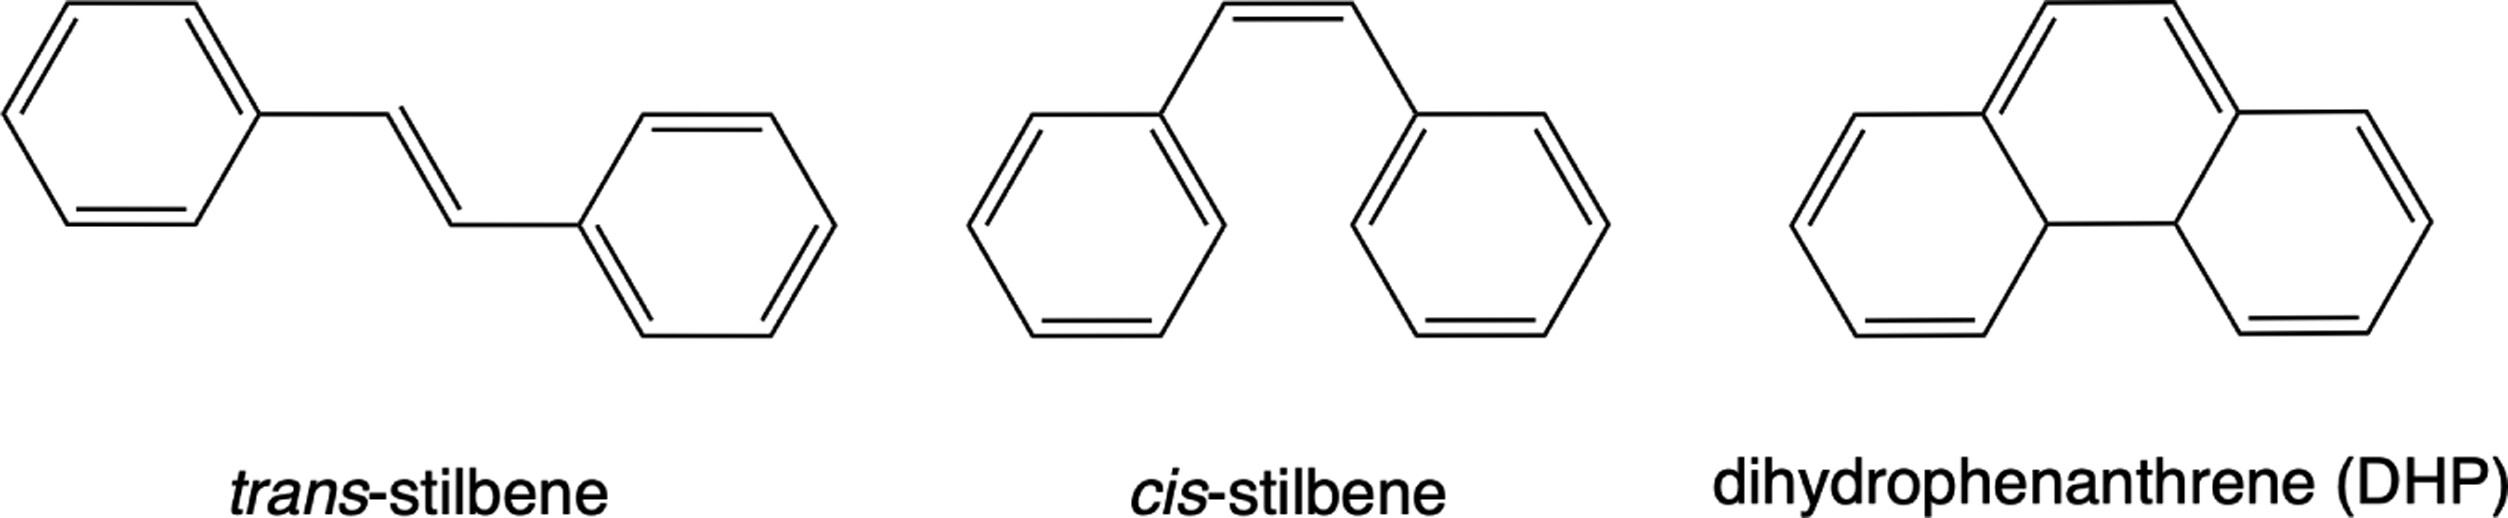
\includegraphics[width=0.9\linewidth]{parts/02-Original_Research_and_Contributions/chapters/02-Primary_Scientific_Contributions/sections/images/images_large_ct4c01008_0001}
\caption{The three stilbene isomers.}
\label{fig:stilbene_isomers}
\end{figure}
The study uses the \gls{fssh} method, described in Sec.~\ref{sec:fewest_switches}, to simulate the nonadiabatic dynamics of \textit{cis}-stilbene using various electronic structure methods. For the low-level method, semiempirical OM3-MRCISD is employed, while for the high-level methods, \gls{sa-casscf} and \gls{sa-caspt2} were used. Using these methods, the study calculates the excited-state lifetimes and populations, quantum yields for photoisomerization and cyclization, and \gls{trpes}. The results are then compared with the experimental data to assess the accuracy of each electronic structure method.
\subsection{Mapping the Potential Energy Surface}
To start the sensitivity analysis, the study first establishes the investigated \gls{pes} and all the important features that influence the photodynamics of \textit{cis}-stilbene. Upon excitation to the first excited state (S$_1$) there are two main relaxation pathways. The first pathway leads through the \textit{cis}-stilbene S$_1$ minimum to an energetically close \gls{ci} between S$_1$ and the ground state (S$_0$) that facilitates the isomerization to \gls{dhp} or back to \textit{cis}-stilbene. The second pathway leads through another S$_1$ minimum to four \glspl{ci} between S$_1$ and S$_0$ that facilitate the isomerization to \textit{trans}-stilbene or back to \textit{cis}-stilbene. Note that all of the \glspl{ci} are energetically accessible from the S$_1$ \gls{fc} region. The \gls{pes} features on all three electronic structure levels are qualitatively similar, with no seemingly preferred pathway. The schematic representation of the \gls{pes} features is shown in Fig.~\ref{fig:pes_features_stilbene}.
\begin{figure}[!ht]
\centering
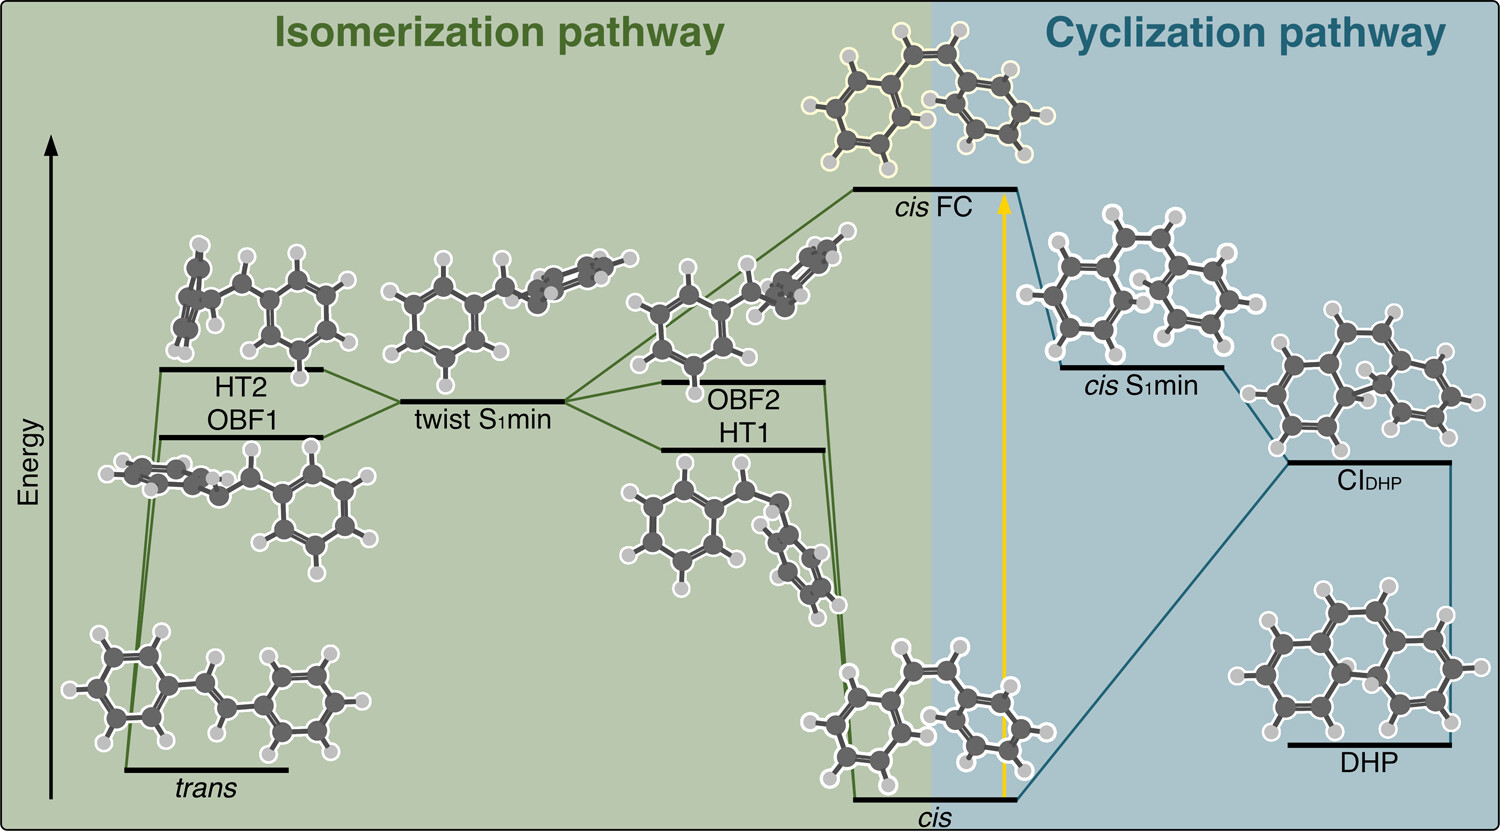
\includegraphics[width=\linewidth]{parts/02-Original_Research_and_Contributions/chapters/02-Primary_Scientific_Contributions/sections/images/images_large_ct4c01008_0003}
\caption{Schematic representation of the \gls{pes} features of \textit{cis}-stilbene relevant to its photodynamics. The diagram illustrates the two main relaxation pathways from the S$_1$ excited state: one leading to the formation of \gls{dhp} via a \gls{ci} accessible from the S$_1$ minimum, and the other leading to \textit{trans}-stilbene via multiple \glspl{ci}.}
\label{fig:pes_features_stilbene}
\end{figure}
\subsection{Nonadiabatic Dynamics Simulations and Results}
After characterizing the stationary points, nonadiabatic dynamics simulations were performed using different electronic structure methods. Quantum yields and excited-state lifetimes obtained from these simulations are summarized in Tab.~\ref{tab:sensitivity_analysis_results}.
\begin{table}[!ht]
\centering
\caption{Summary of the photodynamics results for \textit{cis}-stilbene using different electronic structure methods. The quantum yields for \textit{cis}-stilbene ($\phi_{\symit{cis}}$), \textit{trans}-stilbene ($\phi_{\symit{trans}}$), and \gls{dhp} ($\phi_{\symrm{DHP}}$) formation, along with the excited-state lifetime ($\tau$), are presented. The results from previous studies and experimental data are also included for comparison.}
    \label{tab:sensitivity_analysis_results}
    \begin{tabular}{lcccc}
        \hline
        Level of Theory&$\phi_{\symit{cis}}$&$\phi_{\symit{trans}}$&$\phi_{\symrm{DHP}}$&$\tau$ (fs)\\
        \hline
        OM3-MRCISD(12,17) (LZSH)& $0.48\pm0.05$&$0.52\pm0.05$&$0.00\pm0.00$ &$321\pm10$\\
        SA2-CASSCF/SVP&$0.29\pm0.06$&$0.68\pm0.06$&$0.03\pm0.02$&$360\pm6$\\
        XMS-SA3-CASPT2/cc-pVDZ&$0.55\pm0.14$&$0.02\pm0.04$&$0.43\pm0.14$&$295\pm10$\\
        XMS-SA2-CASPT2/cc-pVDZ&$0.91\pm0.07$&$0.00\pm0.00$&$0.09\pm0.07$&--\\
        \hline
        XMS-SA3-CASPT2(2,2)/cc-pVDZ\supercite{10.1021/jacs.2c12266}&$0.55\pm0.14$&$0.04\pm0.10$&$0.41\pm0.14$& $572\pm16$\\
        OM3-MRCISD(12,17)\supercite{10.1038/s41557-022-01012-0}&0.48&0.52&0.0&$\approx500$\\
        SA2-CASSCF(2,2)/6-31G*\supercite{10.1021/acs.jpcb.0c03344}&$0.45\pm0.04$&$0.52\pm0.04$&$0.04\pm0.01$&$520\pm40$\\
        \hline
        Experiment in Solvents\supercite{10.1021/ja00076a041,10.1021/acs.jpca.8b04011}&0.47-0.59&0.35-0.39&0.05-0.08&380-1650\\
        \hline
    \end{tabular}
\end{table}
The results show significant differences in the quantum yields and excited-state lifetimes depending on the electronic structure method used. The OM3-MRCISD method predicts a nearly equal distribution between \textit{trans}-stilbene and \textit{cis}-stilbene formation, with no \gls{dhp} formation. Whereas the SA2-CASSCF method predicts a higher quantum yield for \textit{trans}-stilbene formation, with a small amount of \gls{dhp} formation. And finally, the XMS-SA3-CASPT2 method predicts a high quantum yield for \gls{dhp} formation, with a low quantum yield for \textit{trans}-stilbene formation. The XMS-SA2-CASPT2 method turns out to be inadequate for describing the photodynamics of \textit{cis}-stilbene, as it predicts almost no population transfer to the ground state. This failure originates from the exclusion of a critical doubly excited state from the state-averaging space. Without the inclusion of this state, the topography of the S$_1$ surface is artificially distorted, creating a deep minimum that traps the wavepacket and prevents it from accessing the \glspl{ci}. Conversely, including this third state in the averaging space (as done in the XMS-SA3-CASPT2 method) corrects the topography, allowing the wavepacket to reach the crossing seams and opening the photocyclization channel.

The excited-state lifetimes also vary, but all methods predict lifetimes comparable to the lower end of the experimental range. The quantum yields in the table above lead to a conclusion that the choice of electronic structure method has a profound impact on the predicted photodynamics. The simple static picture of the \gls{pes} features does not provide enough information to predict the outcome of the dynamics simulations, as all methods show similar \gls{pes} features but yield different photodynamics results.
\subsection{Time-Resolved Photoelectron Spectra}
The study also analyzes the \gls{trpes} obtained from the simulations (Fig.~\ref{fig:stilbene_spectra}) and compares them with experimental data. The \gls{trpes} signal is predominantly sensitive to the initial wavepacket motion out of the \gls{fc} region, rather than the long-time branching ratio at the distant \glspl{ci}. Because all the tested methods (with the exception of the flawed XMS-SA2-CASPT2) predict a very similar initial descent on the S$_1$ surface, their simulated spectra all reasonably match the experimental data. This observation is critical: it demonstrates that agreement with experimental \gls{trpes} alone is insufficient to validate an electronic structure method's ability to accurately predict long-time photoproduct quantum yields.
\begin{figure}[!ht]
\centering
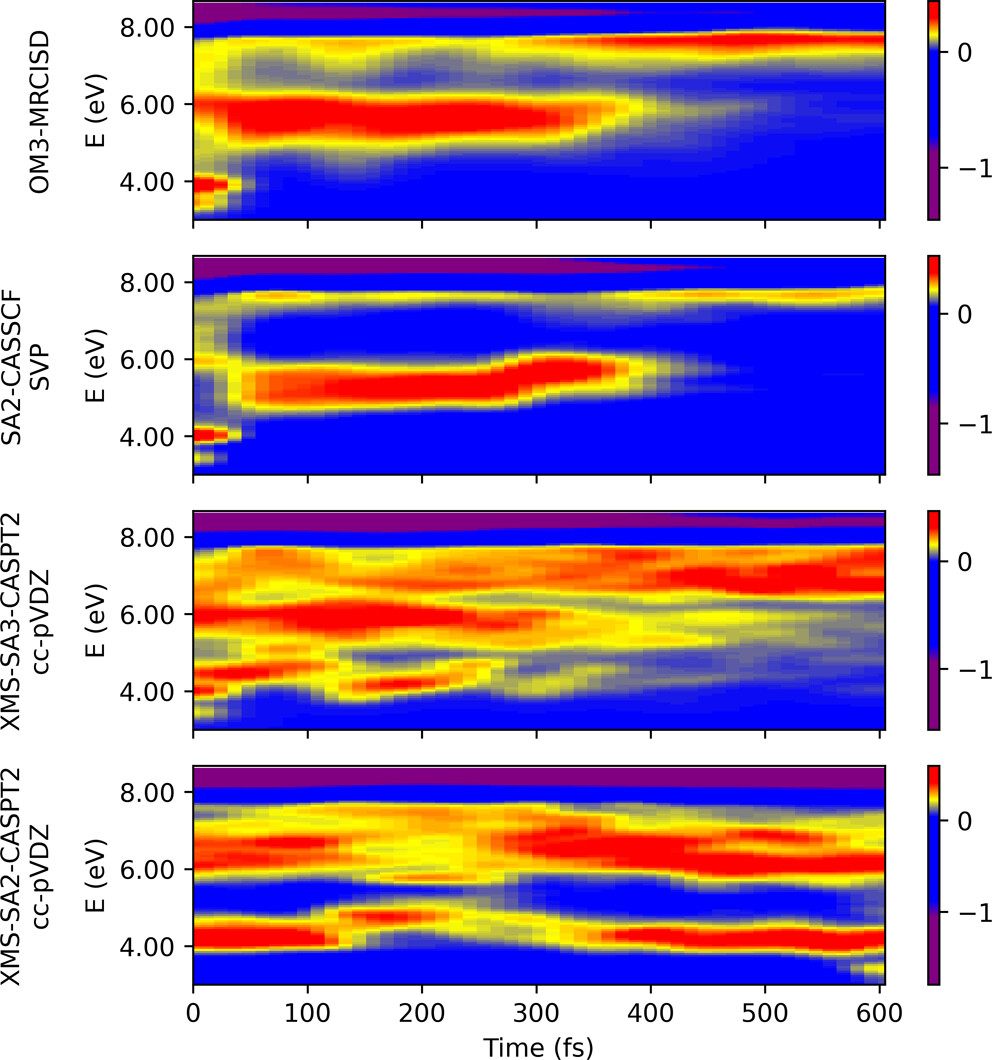
\includegraphics[width=0.7\linewidth]{parts/02-Original_Research_and_Contributions/chapters/02-Primary_Scientific_Contributions/sections/images/images_large_ct4c01008_0009}
\caption{Simulated \gls{trpes} for surface hopping dynamics with various electronic structure methods}
\label{fig:stilbene_spectra}
\end{figure}
Because experimental spectra alone cannot distinguish between various theoretical outcomes, alternative strategies must be utilized to systematically assess the reliability of the underlying electronic structure methods.
\subsection{Nonadiabatic Dynamics Simulations with a Bias Potential}
The drastic differences in quantum yields beg the question: How can we efficiently map the system's sensitivity of nonadiabatic dynamics without the immense computational cost of running trajectories on multiple high-level methods? To explore this, the study introduces an approach where a computationally cheap semiempirical method (OM3-MRCISD) is artificially perturbed to mimic the topographic shifts seen in higher-level methods. 

Specifically, an artificial harmonic bias potential $V_{\text{bias}}=\frac{1}{2}k(r_{ce}-r_{eq})^2$ was added to the central \ce{C=C} bond distance $r_{ce}$, where $k$ is a variable force constant and $r_{eq}$ is the equilibrium bond length. By tuning $k$, the relative energies of the \glspl{ci} can be systematically shifted with respect to the \gls{fc} region without completely recalculating the electronic structure.
\begin{figure}[!ht]
\centering
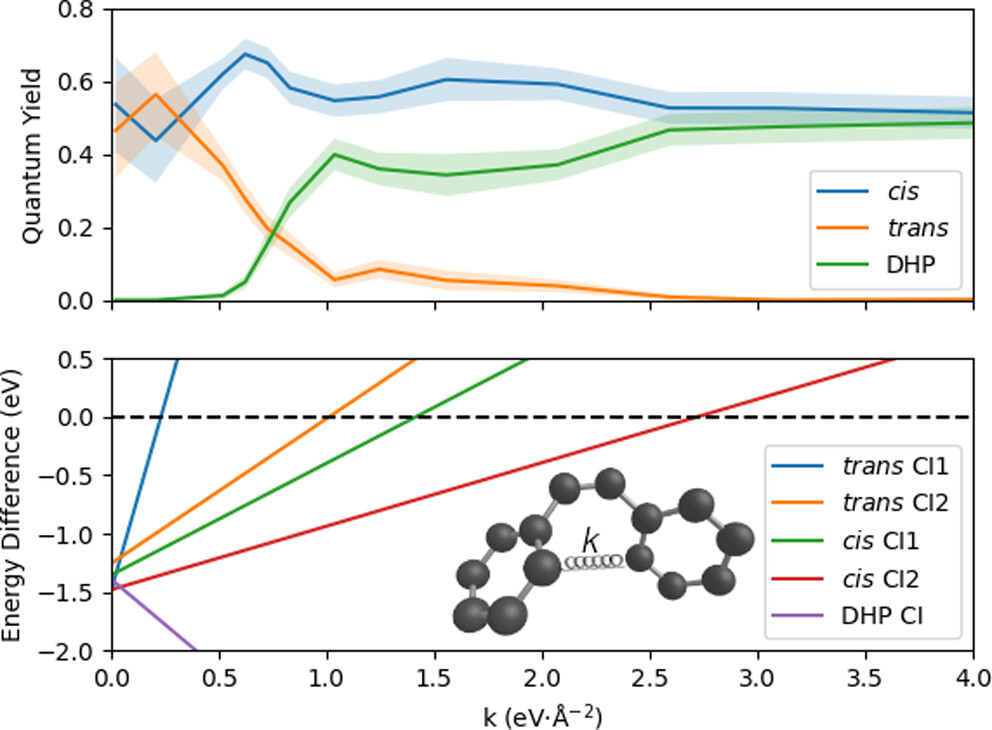
\includegraphics[width=0.7\linewidth]{parts/02-Original_Research_and_Contributions/chapters/02-Primary_Scientific_Contributions/sections/images/images_large_ct4c01008_0011}
\caption{Quantum yields of \textit{cis}-stilbene photoproducts as a function of applied force constant. The upper panel shows the product ratio on the force constant $k$ of the harmonic oscillator, as referenced in the paragraph above. The lower panel shows the energy difference between the \gls{fc} point (dashed line) and several \glspl{ci}, also varying with different values of $k$.}
\label{fig:stilbene_oscillator}
\end{figure}
As shown in Fig.~\ref{fig:stilbene_oscillator}, altering the force constant $k$ directly manipulates the energetic accessibility of the competing pathways. Increasing $k$ effectively raises the energy barrier toward the \textit{trans} pathway. Consequently, the wavepacket is redirected, shifting the population flow to heavily favor the cyclization pathway and yielding more \gls{dhp}. This cleanly demonstrates that even minor energetic shifts on the \gls{pes} can completely invert the macroscopic quantum yields of the reaction.
\subsection{Conclusion}
The investigation of \textit{cis}-stilbene photodynamics demonstrates that the choice of electronic structure method can drastically alter the long-time photoproduct distributions, even when the underlying \gls{pes} features appear qualitatively similar. We learned that the reproducing the short-time dynamics and \gls{trpes} is not sufficient to validate the method's ability to predict the long-time quantum yields. The initial descent from the \gls{fc} region is similar across methods, leading to similar \gls{trpes}, but the branching ratios at the distant \glspl{ci} are highly sensitive to the shape of the \gls{pes} and can vary drastically between methods. By introducing an additional bias potential, we were able to systematically explore how small energetic shifts can completely invert the photoproduct distributions.

In the broader context of this dissertation, these findings emphasize the absolute necessity of algorithmic benchmarking and numerical validation in nonadiabatic dynamics simulations. This work successfully bridges the gap between the purely theoretical analysis of mixed quantum-classical algorithms, as performed in Sec.~\ref{sec:coherence_in_mixed_qc_dynamics}, and the practical application of these algorithms to realistic, highly sensitive photochemical systems.

These findings highlight a critical vulnerability in standard theoretical photochemical workflows. As nonadiabatic dynamics simulations are becoming increasingly common, researchers must be wary of relying on a single comfortable electronic structure method without thorough validation or validating their method solely based on short-time observables. The bias potential approach introduced in this work provides a simple yet powerful tool for assessing the sensitivity of photodynamics outcomes to \gls{pes} features without the need for high-level \textit{ab initio} calculations. By adopting such analyses, the community can gain deeper insights into the relationship between electronic structure and photodynamics, ultimately leading to more reliable predictions and a better understanding of complex photochemical processes.

\section{Curvature-Driven Surface Hopping Algorithms}\label{sec:curvature_driven_surface_hopping_algorithms}
\textit{Commentary on: \fullcite{10.1021/acs.jctc.5c01176}}

The second published work of this thesis focuses on curvature-driven surface hopping algorithms from article \textit{Curvature-Driven Nonadiabatic Dynamics without Explicit Nonadiabatic Couplings} in \textit{Journal of Chemical Theory and Computation}. All simulations on model potentials in this work were performed using custom-built \textsc{Zinq} package.\supercite{10.5281/zenodo.18386143}

When performing nonadiabatic dynamics simulations, one has several options how to treat the nonadiabatic transitions between electronic states. The most common approach is to use surface hopping methods, where classical nuclear trajectories evolve on \glspl{pes} and can hop between them based on certain criteria. The most widely used surface hopping method is the \gls{fssh} method, described in Sec.~\ref{sec:fewest_switches}, which relies on the calculation of \gls{tdc} to propagate the electronic wavefunction in adiabatic basis. Details about the \gls{tdc} can be found in Sec.~\ref{sec:time_derivative_coupling} and the adiabatic basis is described in Sec.~\ref{sec:adiabatic_vs_diabatic_representation}. From quantum-chemical calculations, the \gls{tdc} is usually obtained using \gls{nacv} (Eq.~\eqref{eq:tdc_nacv}) that are computationally expensive to calculate and not available for all electronic structure methods. The question arises whether it is possible to perform nonadiabatic dynamics simulations without the need to calculate \gls{nacv} at all.

One of the fairly known approaches to avoid the calculation of \gls{tdc} is to use the \gls{lzsh}, described in depth in Sec.~\ref{sec:landau_zener}, which estimates the hopping probabilities based on the exact solution of a two-level system with linearly varying diabatic energies and constant diabatic coupling. The \gls{lzsh} method has been successfully applied in various nonadiabatic dynamics simulations, but it is not as popular as the \gls{fssh} method due to its theoretical limitations and fairly recent applications to simulations in adiabatic basis. Since most of the quantum-dynamical codes already provide \gls{fssh} implementation, it would be beneficial to have a method that can be easily incorporated into existing \gls{fssh} frameworks without the need to calculate \gls{nacv} from \textit{ab initio} methods.

The study presented in this article aims to evaluate the performance of the newly proposed curvature-driven $\kappa$\gls{fssh} method in comparison to the traditional \gls{fssh} and \gls{lzsh} methods. The theory behind the $\kappa$\gls{fssh} method is described in detail in Sec.~\ref{sec:baeck_an}. The surface hopping methods are tested on several one-dimensional model systems, including single avoided crossing, three-state crossing and models exhibiting trivial crossings. After the one-dimensional models, the study applies the algorithm to more realistic systems as 8-dimensional model of uracil cation or nonadiabatic dynamics of stilbene, azobenzene or cyclobutanone. In the simulations, the quantities of interest are the state populations and the magnitude of the \gls{tdc}. The populations obtained from the surface hopping methods are compared to the numerically exact quantum dynamics results (Sec.~\ref{sec:split_operator_method}), while the \gls{tdc} values are compared to those calculated from the \gls{npi} algorithm described in Sec.~\ref{sec:norm_preserving_interpolation}. The study also introduces a modified version of the $\kappa$\gls{fssh} method, called $\lambda$\gls{fssh}, which should theoretically be more accurate in predicting the \gls{tdc} values (Eq.~\eqref{eq:lambda_tdc}).

Since the standard \gls{lzsh} algorithm is strictly formulated for two-level systems, applying it to environments with three-state crossings requires theoretical extensions. To address this, the study introduces two generalized multistate variants: the maximum curvature version (\gls{lzsh}$_{\symrm{maxcurv}}$) and the nearest state version (\gls{lzsh}$_{\symrm{nearest}}$). When a multistate crossing is identified, the \gls{lzsh}$_{\symrm{maxcurv}}$ algorithm computes transition probabilities only to the state exhibiting the maximum second derivative of the energy gap ($\ddot{Z}_{ik}$), operating on the physical premise that strongly interacting states will exhibit the sharpest curvature. Alternatively, the \gls{lzsh}$_{\symrm{nearest}}$ variant restricts population transfer strictly to the energetically closest state. Both variants are critically evaluated alongside the curvature-driven \gls{fssh} schemes.
\subsection{Simulations on Model Systems}
The results from the simulations on a single avoided crossing model in Fig.~\ref{fig:curvature_single_avoided_crossing} show that the $\kappa$\gls{fssh} already performs significantly worse than the traditional \gls{fssh} and \gls{lzsh} methods in terms of state populations. Inspecting the \gls{tdc} in this case reveals that the $\kappa$\gls{fssh} method produces a narrower peak compared to the reference \gls{npi} values, which likely contributes to the poorer performance in state populations.
\begin{figure}[!ht]
\centering
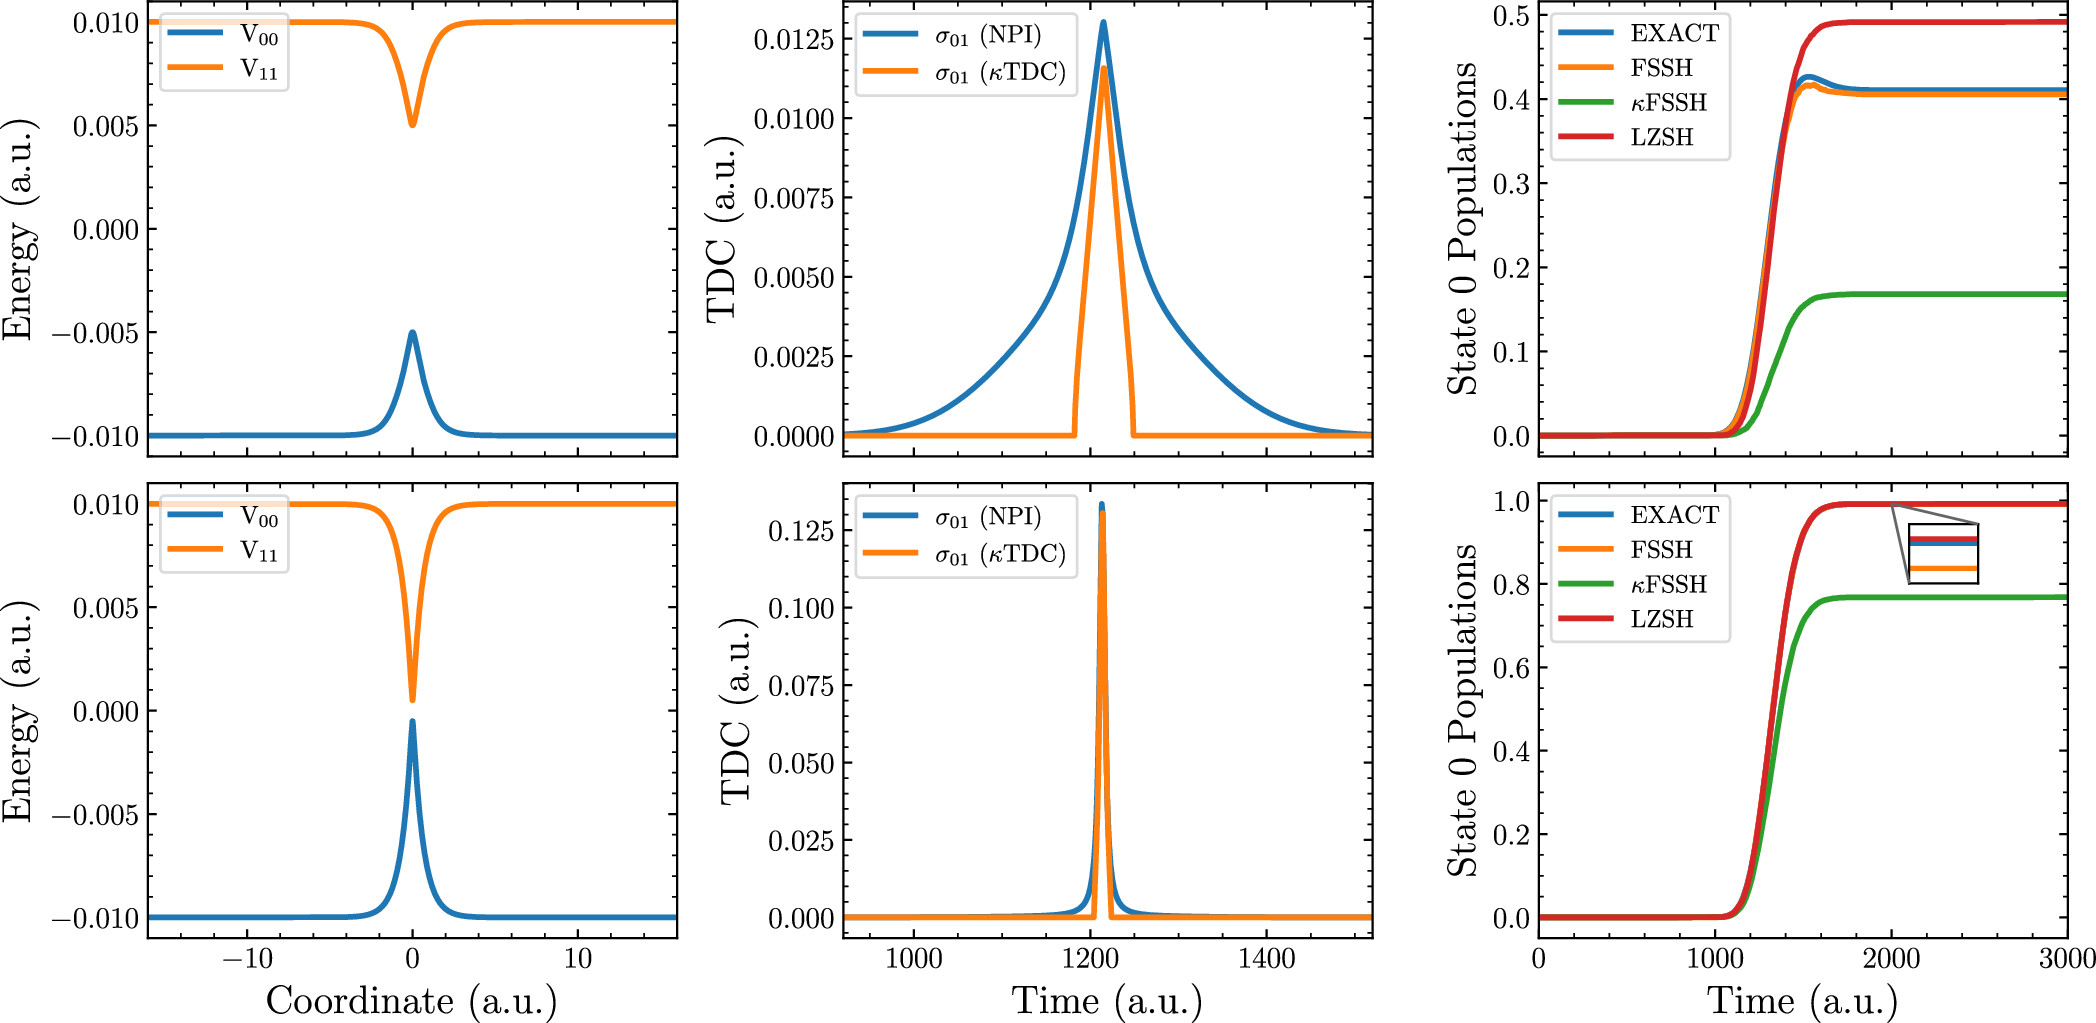
\includegraphics[width=\linewidth]{parts/02-Original_Research_and_Contributions/chapters/02-Primary_Scientific_Contributions/sections/images/images_large_ct5c01176_0002}
\caption{Nonadiabatic dynamics simulations on Tully’s Simple Avoided Crossing potential defined using two different sets of diabatic coupling constants. Reproduced from Ref.~\cite{10.1021/acs.jctc.5c01176} under \href{https://creativecommons.org/licenses/by/4.0}{CC BY 4.0}.}
\label{fig:curvature_single_avoided_crossing}
\end{figure}
In the three-state crossing model (Fig.~\ref{fig:curvature_three-state_crossing}), the performance of the $\kappa$\gls{fssh} method is even more unsatisfactory. The fundamental flaw of the curvature-driven approach becomes apparent here: because $\kappa$\gls{fssh} relies solely on the adiabatic energy gap ($Z_{ik}$) and its temporal derivatives, it assigns non-zero \gls{tdc} values between any states that are energetically close, even if their wavefunctions are strictly orthogonal and no physical coupling exists. For instance, while the reference \gls{npi} method correctly predicts zero coupling between states 0 and 2, $\kappa$\gls{fssh} artificially forces population transfer between them, leading to unphysical trajectory outcomes.
\begin{figure}[!ht]
\centering
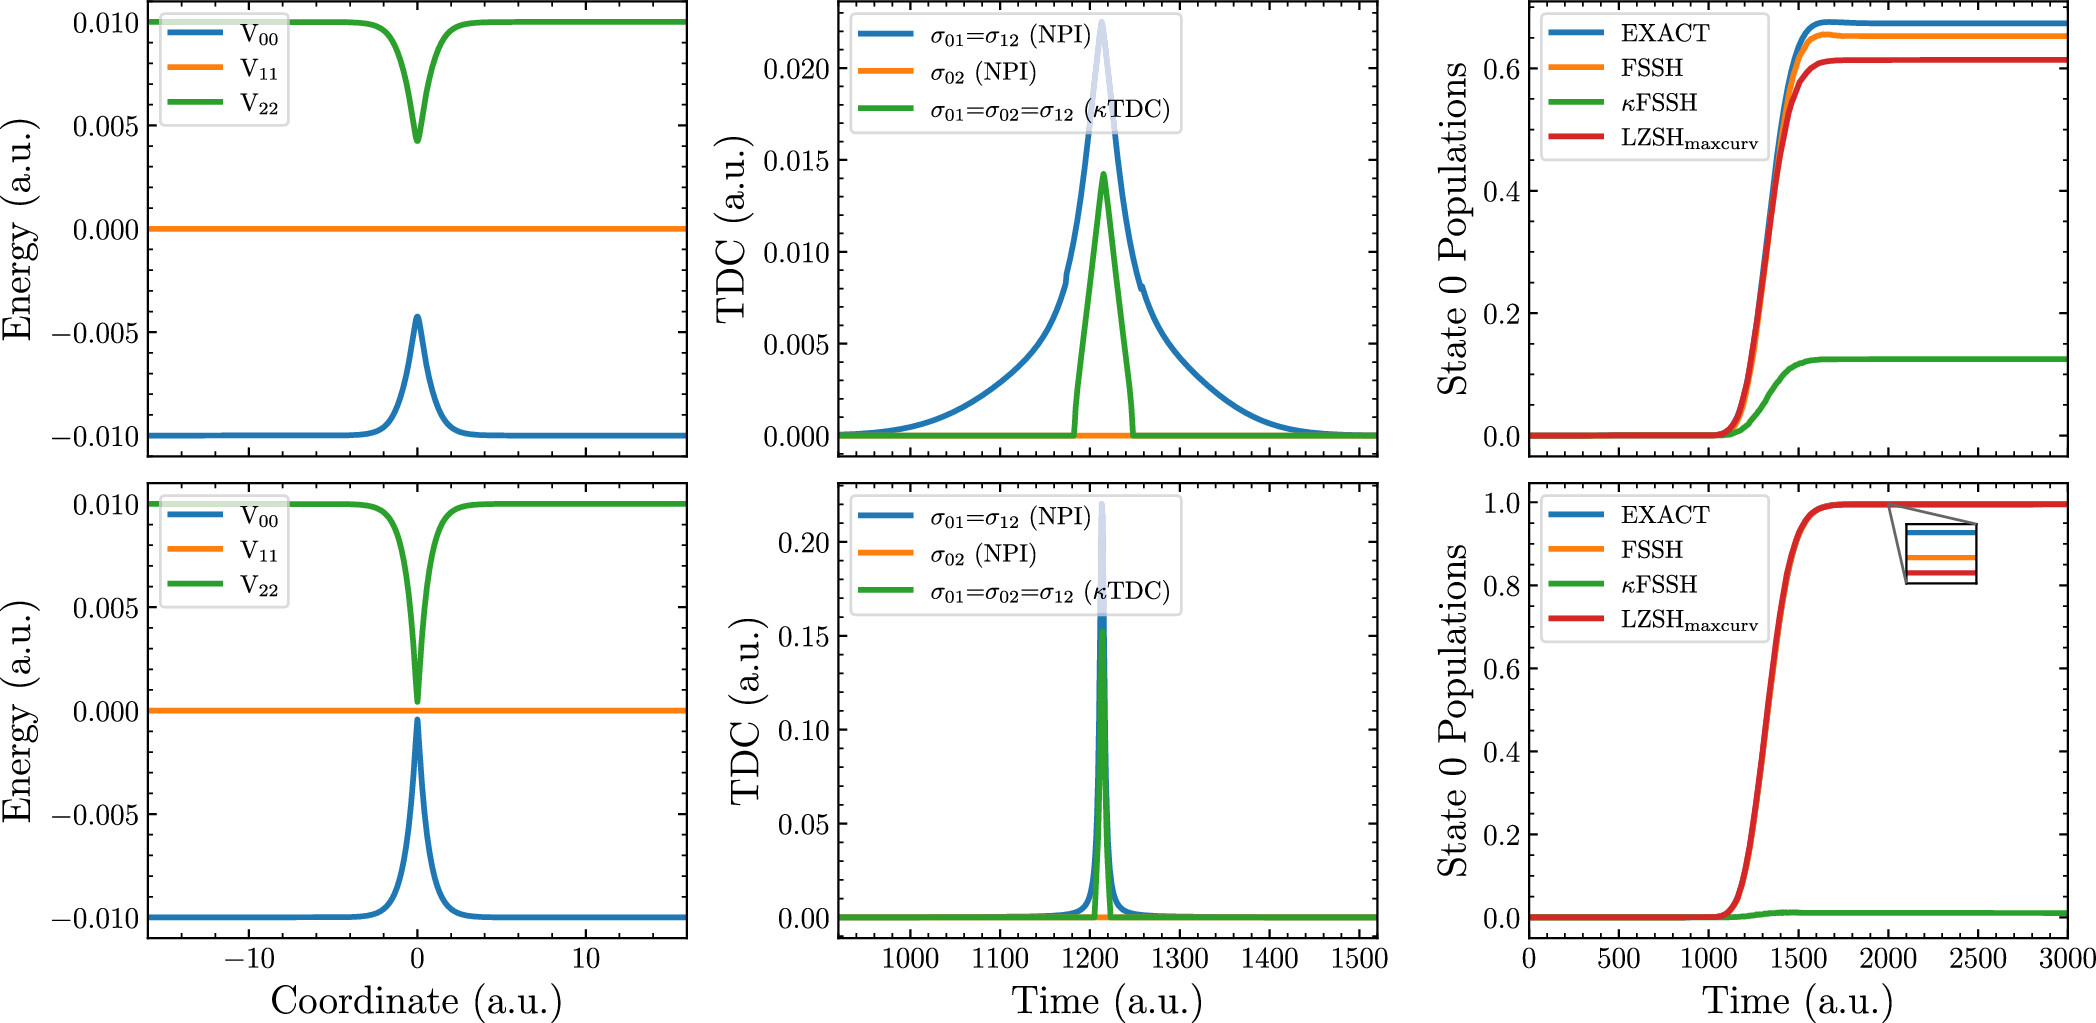
\includegraphics[width=\linewidth]{parts/02-Original_Research_and_Contributions/chapters/02-Primary_Scientific_Contributions/sections/images/images_large_ct5c01176_0003}
\caption{Nonadiabatic dynamics simulations on three-state crossing potential defined using two different sets of diabatic coupling constants. Reproduced from Ref.~\cite{10.1021/acs.jctc.5c01176} under \href{https://creativecommons.org/licenses/by/4.0}{CC BY 4.0}.}
\label{fig:curvature_three-state_crossing}
\end{figure}
Moving on to the trivial crossing models (Fig.~\ref{fig:curvature_trivial_crossing}), the $\kappa$\gls{fssh} method again fails to reproduce the correct state populations, while the traditional \gls{fssh} and \gls{lzsh} methods perform without issues. At a trivial crossing, the true \gls{nacv} theoretically approaches a singularity (a Dirac delta function), necessitating a complete 100\% population transfer. However, investigating the \gls{tdc} values reveals that the analytical form of the $\kappa$\gls{fssh} and $\lambda$\gls{fssh} approximations fundamentally caps the maximum coupling magnitude, producing a finite, broadened peak instead of a singularity. This insufficient coupling magnitude traps residual population in the excited state.
\begin{figure}[!ht]
\centering
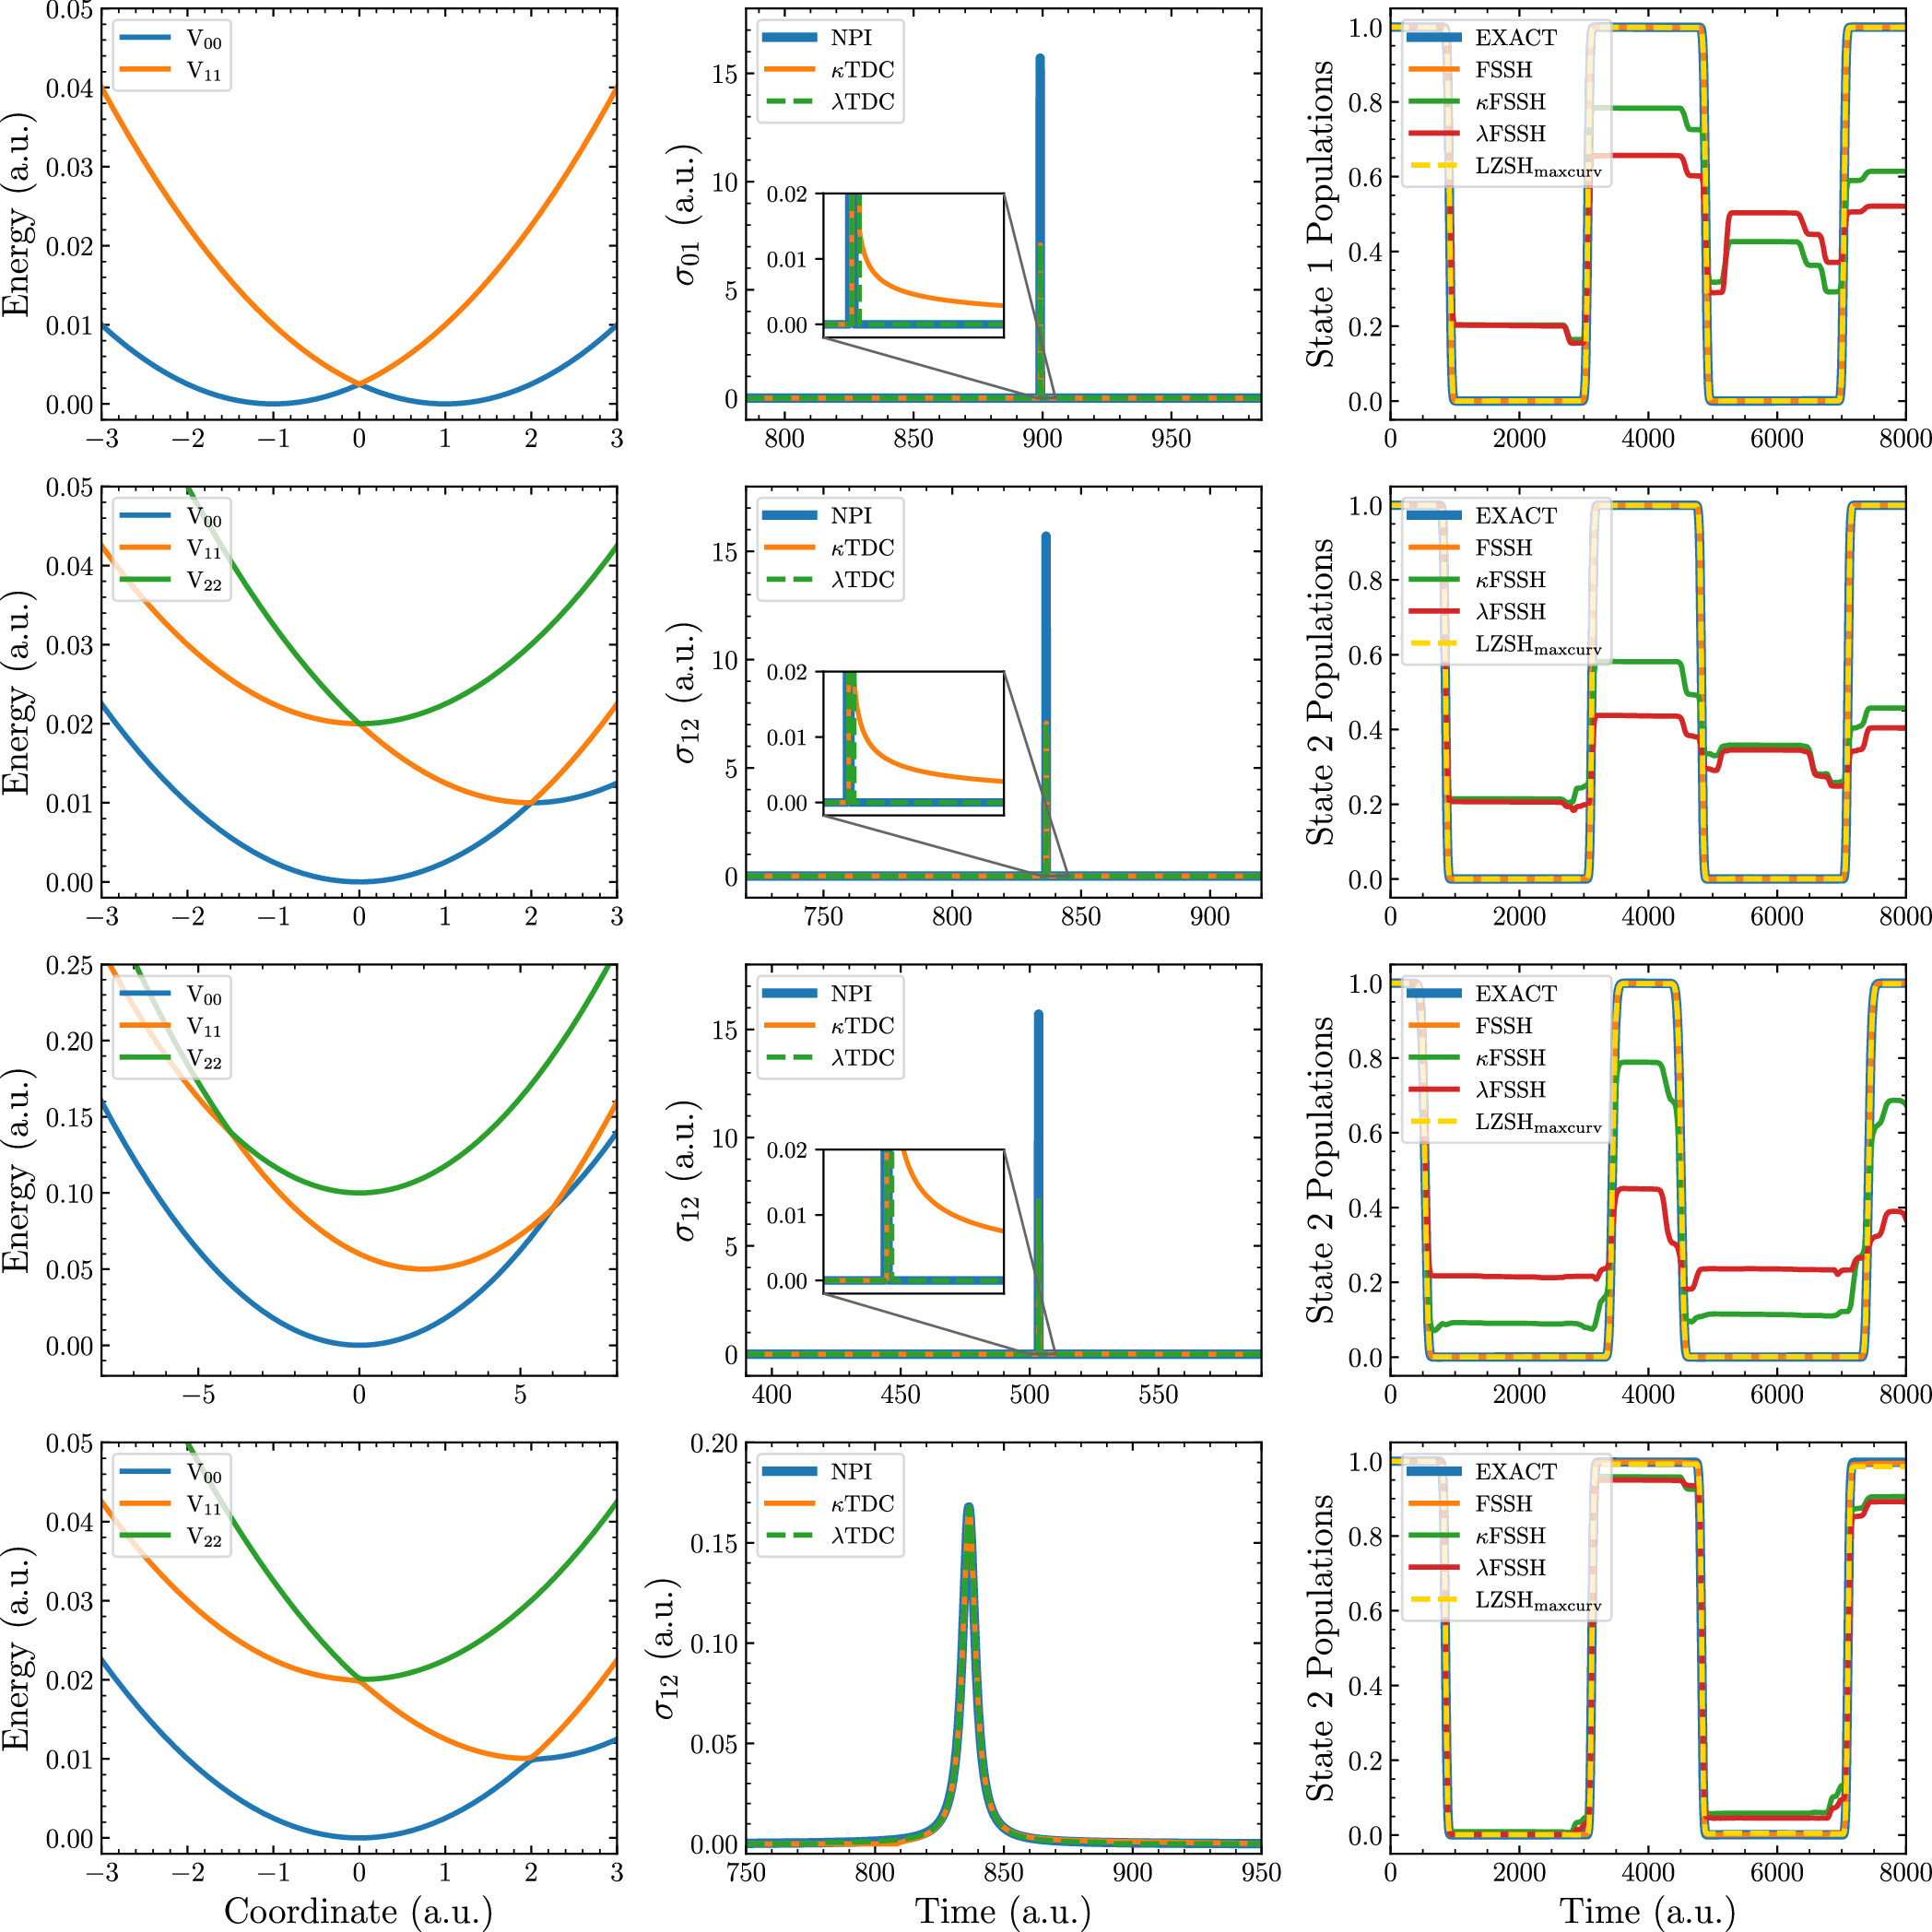
\includegraphics[width=\linewidth]{parts/02-Original_Research_and_Contributions/chapters/02-Primary_Scientific_Contributions/sections/images/images_large_ct5c01176_0004}
\caption{Nonadiabatic dynamics simulations on trivial crossing models. Reproduced from Ref.~\cite{10.1021/acs.jctc.5c01176} under \href{https://creativecommons.org/licenses/by/4.0}{CC BY 4.0}.}
\label{fig:curvature_trivial_crossing}
\end{figure}
\subsection{Vibronic Coupling Model of Uracil Cation}
Applying the algorithms to the 8-dimensional vibronic coupling model of the uracil cation, the failures of the $\kappa$\gls{fssh} method seen in 1D models are somewhat dampened, as seen in Fig.~\ref{fig:curvature_uracil}. It turns out that working in eight dimensions is actually quite forgiving for the algorithm, even if it is completely unforgiving for the human attempting to mentally visualize the crossing seams. \gls{fssh}, \gls{lzsh}, and $\kappa$\gls{fssh} all qualitatively capture the ultrafast relaxation. This suggests that the complex topology of multidimensional crossing seams can be more forgiving than strict 1D models. However, quantitative discrepancies remain visible: while the reference \gls{fssh} correctly predicts negligible population transfer to the $D_3$ state, the curvature-driven approaches inaccurately leak population into $D_3$, once again indicating a structural limitation in capturing the correct coupling mechanisms in densely packed state manifolds.
\begin{figure}[!ht]
\centering
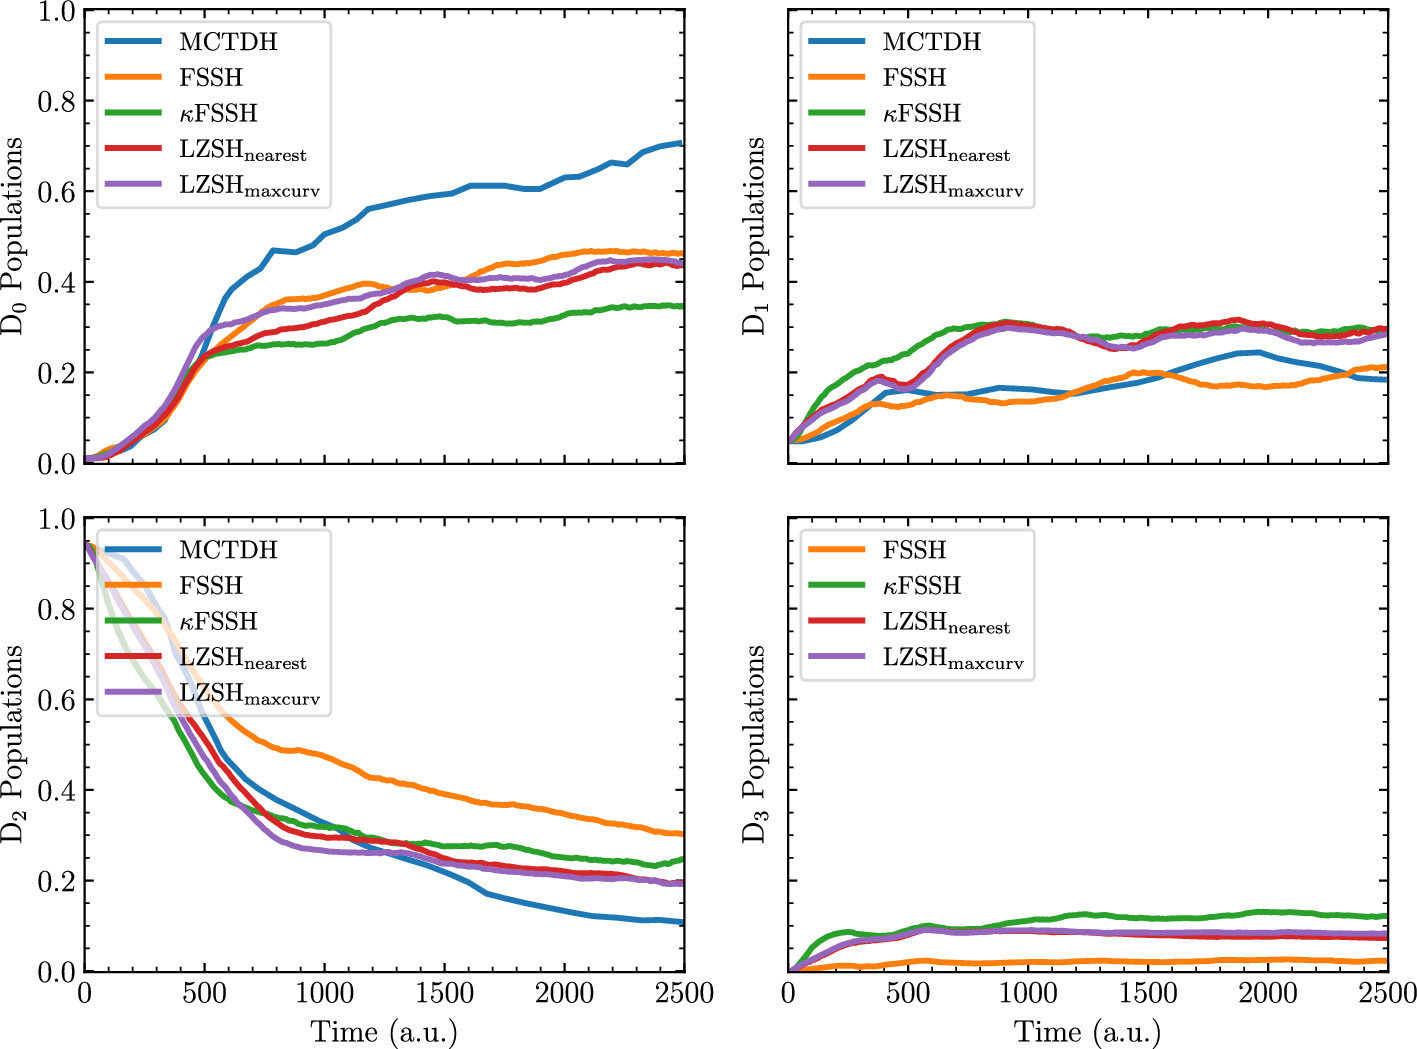
\includegraphics[width=\linewidth]{parts/02-Original_Research_and_Contributions/chapters/02-Primary_Scientific_Contributions/sections/images/images_large_ct5c01176_0005}
\caption{Nonadiabatic dynamics simulations on vibronic coupling model of uracil cation. Reproduced from Ref.~\cite{10.1021/acs.jctc.5c01176} under \href{https://creativecommons.org/licenses/by/4.0}{CC BY 4.0}.}
\label{fig:curvature_uracil}
\end{figure}
\subsection{Simulations on Realistic Systems}
The most severe limitations of curvature-driven methods emerge when applied to on-the-fly \textit{ab initio} simulations of real molecules like \textit{cis}-stilbene, \textit{trans}-azobenzene (Fig.~\ref{fig:curvature_stilbene}), and cyclobutanone. In these realistic systems, multireference electronic structure calculations (like OM3-MRCISD or CASSCF) frequently yield \glspl{pes} with small, localized discontinuities due to orbital rotations into the active space or state-averaging root flipping. 

Because the $\kappa$\gls{fssh} method depends directly on the second time-derivative of the energy gap ($\ddot{Z}_{ik}$), even a microscopic discontinuity in the \gls{pes} causes the numerical second derivative to explode. This translates into erratic spikes in the simulated \gls{tdc}, triggering continuous spurious hops and entirely corrupting the state populations. 

To salvage trajectory stability in such environments, this study introduced a novel discontinuity-blocking algorithm for the \gls{lzsh} method. When the \gls{lzsh} algorithm detects a minimum in the energy gap, it computes a ratio ($\alpha$) of the numerical second derivatives at the current and previous time steps. True avoided crossings exhibit smooth variations in curvature ($\alpha<0.3$), whereas discontinuities trigger abrupt changes ($\alpha>1.3$). By dynamically blocking hops when $\alpha>1.3$, the modified \gls{lzsh} algorithm successfully navigates rough \textit{ab initio} surfaces where $\kappa$\gls{fssh} fails, as evidenced by its strong agreement with standard \gls{fssh} in Fig.~\ref{fig:curvature_stilbene}.
\begin{figure}[!ht]
\centering
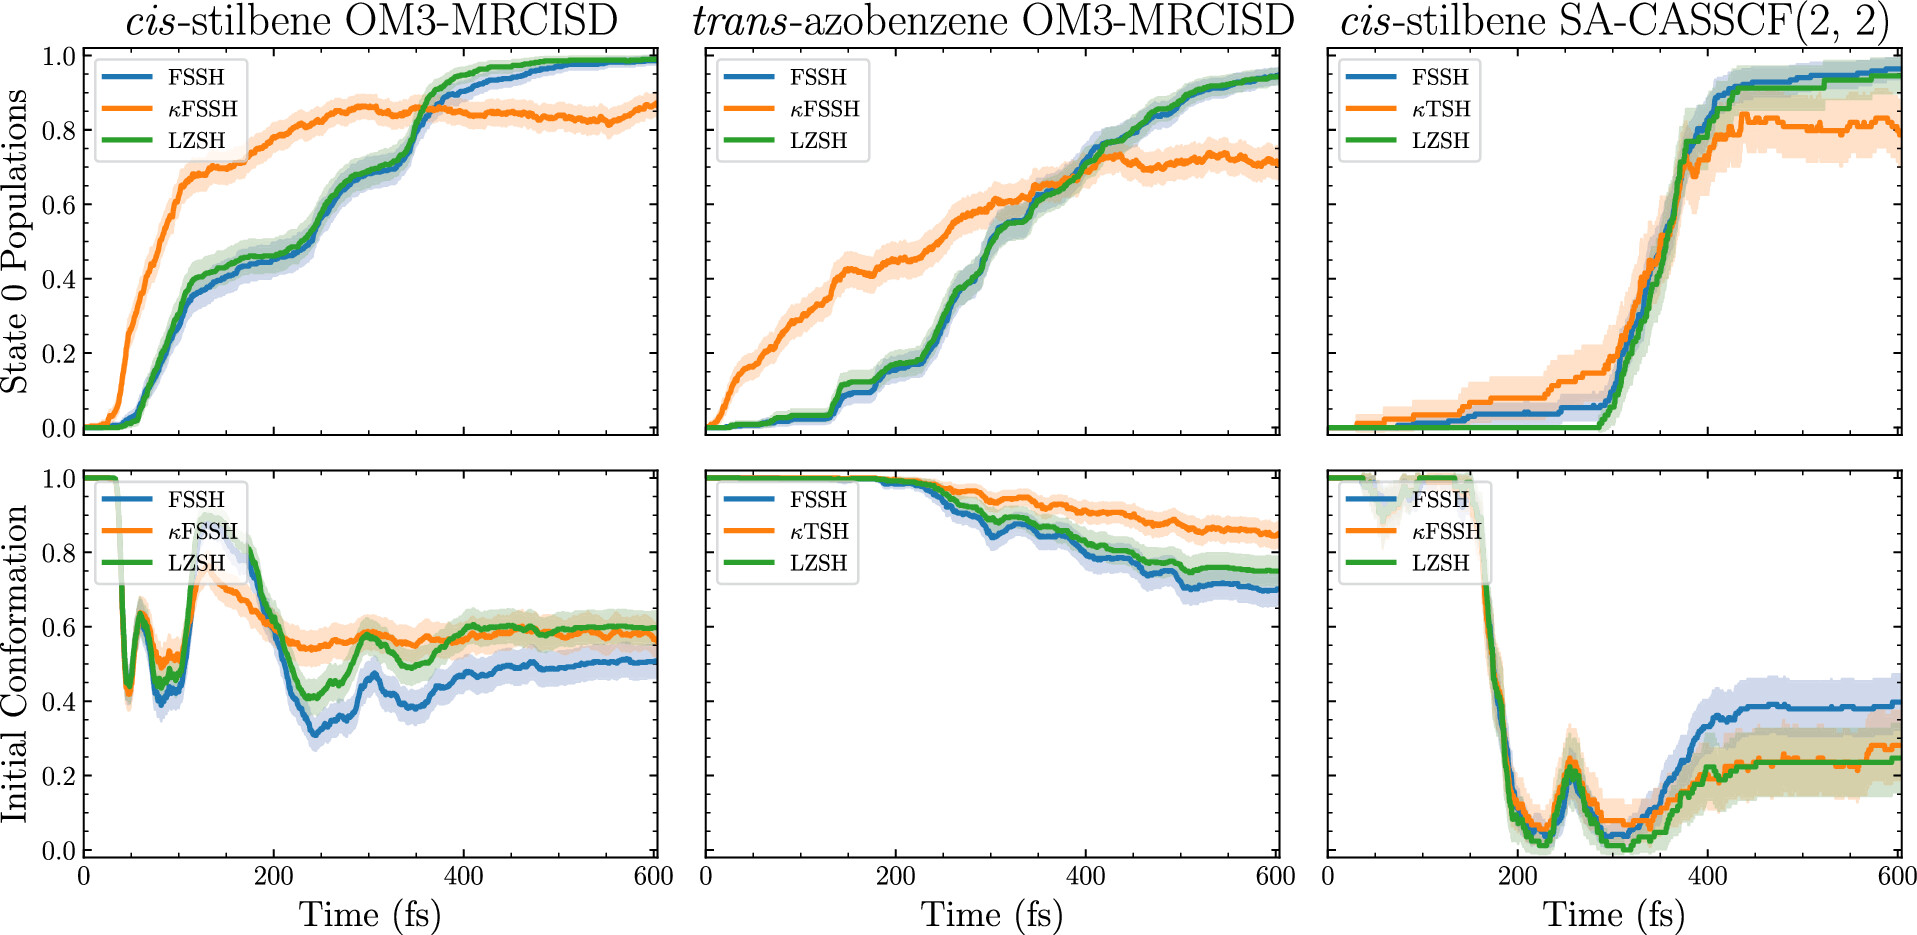
\includegraphics[width=\linewidth]{parts/02-Original_Research_and_Contributions/chapters/02-Primary_Scientific_Contributions/sections/images/images_large_ct5c01176_0006}
\caption{Nonadiabatic dynamics simulations on \textit{cis}-stilbene and \textit{trans}-azobenzene. Reproduced from Ref.~\cite{10.1021/acs.jctc.5c01176} under \href{https://creativecommons.org/licenses/by/4.0}{CC BY 4.0}.}
\label{fig:curvature_stilbene}
\end{figure}
\subsection{Conclusion}
The study presented here provides a comprehensive evaluation of the curvature-driven $\kappa$\gls{fssh} method against traditional \gls{fssh} and \gls{lzsh} approaches across a spectrum of model systems and realistic molecular simulations. Ultimately, we learned that while bypassing the need for \gls{nacv} by relying solely on the curvature of the adiabatic energy gap is an appealing shortcut, it suffers from significant limitations. In idealized 1D models, the $\kappa$\gls{fssh} method completely fails to reproduce correct state populations and \gls{tdc} values, particularly in systems with trivial crossings. More importantly, severe breakdowns also occur in realistic on-the-fly \textit{ab initio} simulations of molecules like \textit{cis}-stilbene and \textit{trans}-azobenzene, where the presence of discontinuities in the \glspl{pes} leads to erratic spikes in the \gls{tdc} and unphysical population transfer. In contrast, the traditional \gls{fssh} and \gls{lzsh} methods consistently outperform the curvature-driven approach in terms of state populations and \gls{tdc} values across all tested systems.

In the broader context of this thesis, these findings validate the numerical benchmarking and exact quantum dynamics framework (developed via the custom \textsc{Zinq} package) detailed in studies in Chapter~\ref{chp:supporting_numerical_studies}. Furthermore, to improve the \gls{lzsh} method's robustness in realistic \textit{ab initio} simulations, we introduced a novel discontinuity-blocking algorithm that successfully navigates rough \glspl{pes} where $\kappa$\gls{fssh} fails. Future research may focus on refining the curvature-driven algorithms to enhance their accuracy and reliability in nonadiabatic dynamics simulations, while also exploring specific applications where the $\kappa$\gls{fssh} method could still be useful despite its limitations.

This study provides two primary contributions to the application of nonadiabatic dynamics. First, they inform the computational chemistry community that algorithms relying on the curvature of the adiabatic energy gap are inherently incompatible with noisy or discontinuous \glspl{pes}, which are common in realistic \textit{ab initio} simulations. Second, it delivers a highly practical solution in the form of a discontinuity-blocking and 3-state-crossing-compatible variation of the \gls{lzsh} algorithm, which can be easily implemented in existing quantum chemistry codes to enhance the robustness of nonadiabatic dynamics simulations without the need for \gls{nacv}.

\section{Spin-Orbit Induced Charge Transfer}\label{sec:spin_orbit_induced_charge_transfer}
\textit{Commentary on: \fullcite{10.1016/j.jqsrt.2025.109697}}

The next published work of this thesis focuses on spin-orbit induced charge transfer from article \textit{Spin--Orbit Induced Charge Transfer in \ce{H^+}/\ce{D^+}/\ce{T^+}-\ce{N(^4S)} Collisions} in \textit{Journal of Quantitative Spectroscopy and Radiative Transfer}. All quantum dynamical simulations in this work were performed by custom built \textsc{Zinq} package.\supercite{10.5281/zenodo.18386143}

The study focuses on the investigation of charge transfer processes in collisions between protons (\ce{H^+}), deuterons (\ce{D^+}), tritons (\ce{T^+}) and nitrogen atoms in their ground state (\ce{N}($^4$S)). Understanding these specific collision dynamics is critical for astrophysical modeling (such as the heliosphere and molecular clouds) and for optimizing magnetic confinement fusion plasmas. For instance, nitrogen impurity seeding is routinely modeled in transport codes like SOLPS-ITER to cool the plasma edge, making accurate data for heavier hydrogen isotopes (deuterium and tritium) essential. Historically, the spin-orbit induced charge transfer for this system was investigated over 30 years ago using only approximate potentials.
\subsection{Background Theory and Computational Details}
In the context of nonadiabatic dynamics simulations, the accurate description of \acrfull{soc} is often challenging, especially when combined with the need to cover a wide range of collision energies. The study presented in this article aims to modernize this data by employing a combination of high-level quantum-mechanical calculations, \acrfull{lz} theory, and an efficient 1D/2D nonadiabatic wavepacket dynamics scheme to rigorously investigate the \ce{N(^4S) + H^+ -> N^+(^3P) + H(^2S)} reaction.

To calculate the cross sections, the study first computes the \acrshort{pes} for the relevant electronic states ($^4\Sigma$ and $^2\Pi$) using the highly accurate MRCI/aug-cc-pVQZ-F12 level of theory. A unique, peculiar feature of this system is that after the crossing point ($r_x=2.19$ Bohr), the potential energy curves remain remarkably close together at short internuclear distances. Concurrently, the calculated \acrshort{soc} matrix elements exhibit a massive increase in this short-range region, peaking near 0.2 Bohr. Because this strong, short-range coupling significantly influences high-energy collisions, simple curve-crossing models are insufficient.

To capture this without the immense computational cost of full 3D wavepacket dynamics, the study introduces a highly efficient methodology mapping 1D dynamics to 3D scattering. 1D quantum dynamics simulations are performed at a zero impact parameter ($b=0$) using the custom \textsc{Zinq} package. By exploiting the relationship between collision energy $E$ and the impact parameter $b$ within the \acrshort{lz} framework, the 1D charge transfer probability $P(E)$ can be analytically transformed to simulate non-zero impact parameters via an effective energy as
\begin{equation}
P(E,b)=P\left(E-\frac{b^2E}{r_x^2}\right).
\end{equation}
This transformation allows for the rapid calculation of 3D cross sections $\sigma(E)$ entirely from 1D quantum dynamics simulations. Validation against full 2D and 3D quantum scattering results is included in the supporting information of the article, confirming the robustness of this dimension-reduction technique at high energies. Using these transformed charge transfer probabilities, the 3D scattering cross sections are calculated by integrating over the impact parameter as
\begin{equation}
\sigma(E)=2\pi\int_0^{(1-\frac{E_x}{E})r_x}bP(E,b)\symrm{d}b,
\end{equation}
where $E_x$ is the activation energy for the charge transfer process and $r_x$ is the crossing point between the relevant \acrshort{pes}.
\subsection{Scattering Cross Sections and Rate Constants}
The calculated cross sections from 1D quantum dynamics (WP) and \acrshort{lz} theory are presented in Fig.~\ref{fig:soc_charge_transfer_cross_sections}. For brevity, only the results for the \ce{N-D^+} and \ce{N-T^+} systems are shown here. The results reveal two critical physical insights. First, at low to moderate energies, both methods yield similar cross sections, confirming the validity of \acrshort{lz} theory for the primary crossing event. However, at high collision energies, the wavepacket cross sections diverge and become distinctly larger than the \acrshort{lz} predictions. This deviation is physically driven by the wavepacket accessing the short-range region where the \acrshort{soc} is drastically enhanced. Second, there is a pronounced isotope effect in the cross sections, with the heavier tritium and deuterium isotopes yielding larger cross sections than hydrogen.
\begin{figure}[!ht]
\centering
\begin{subfigure}{.5\textwidth}
\centering
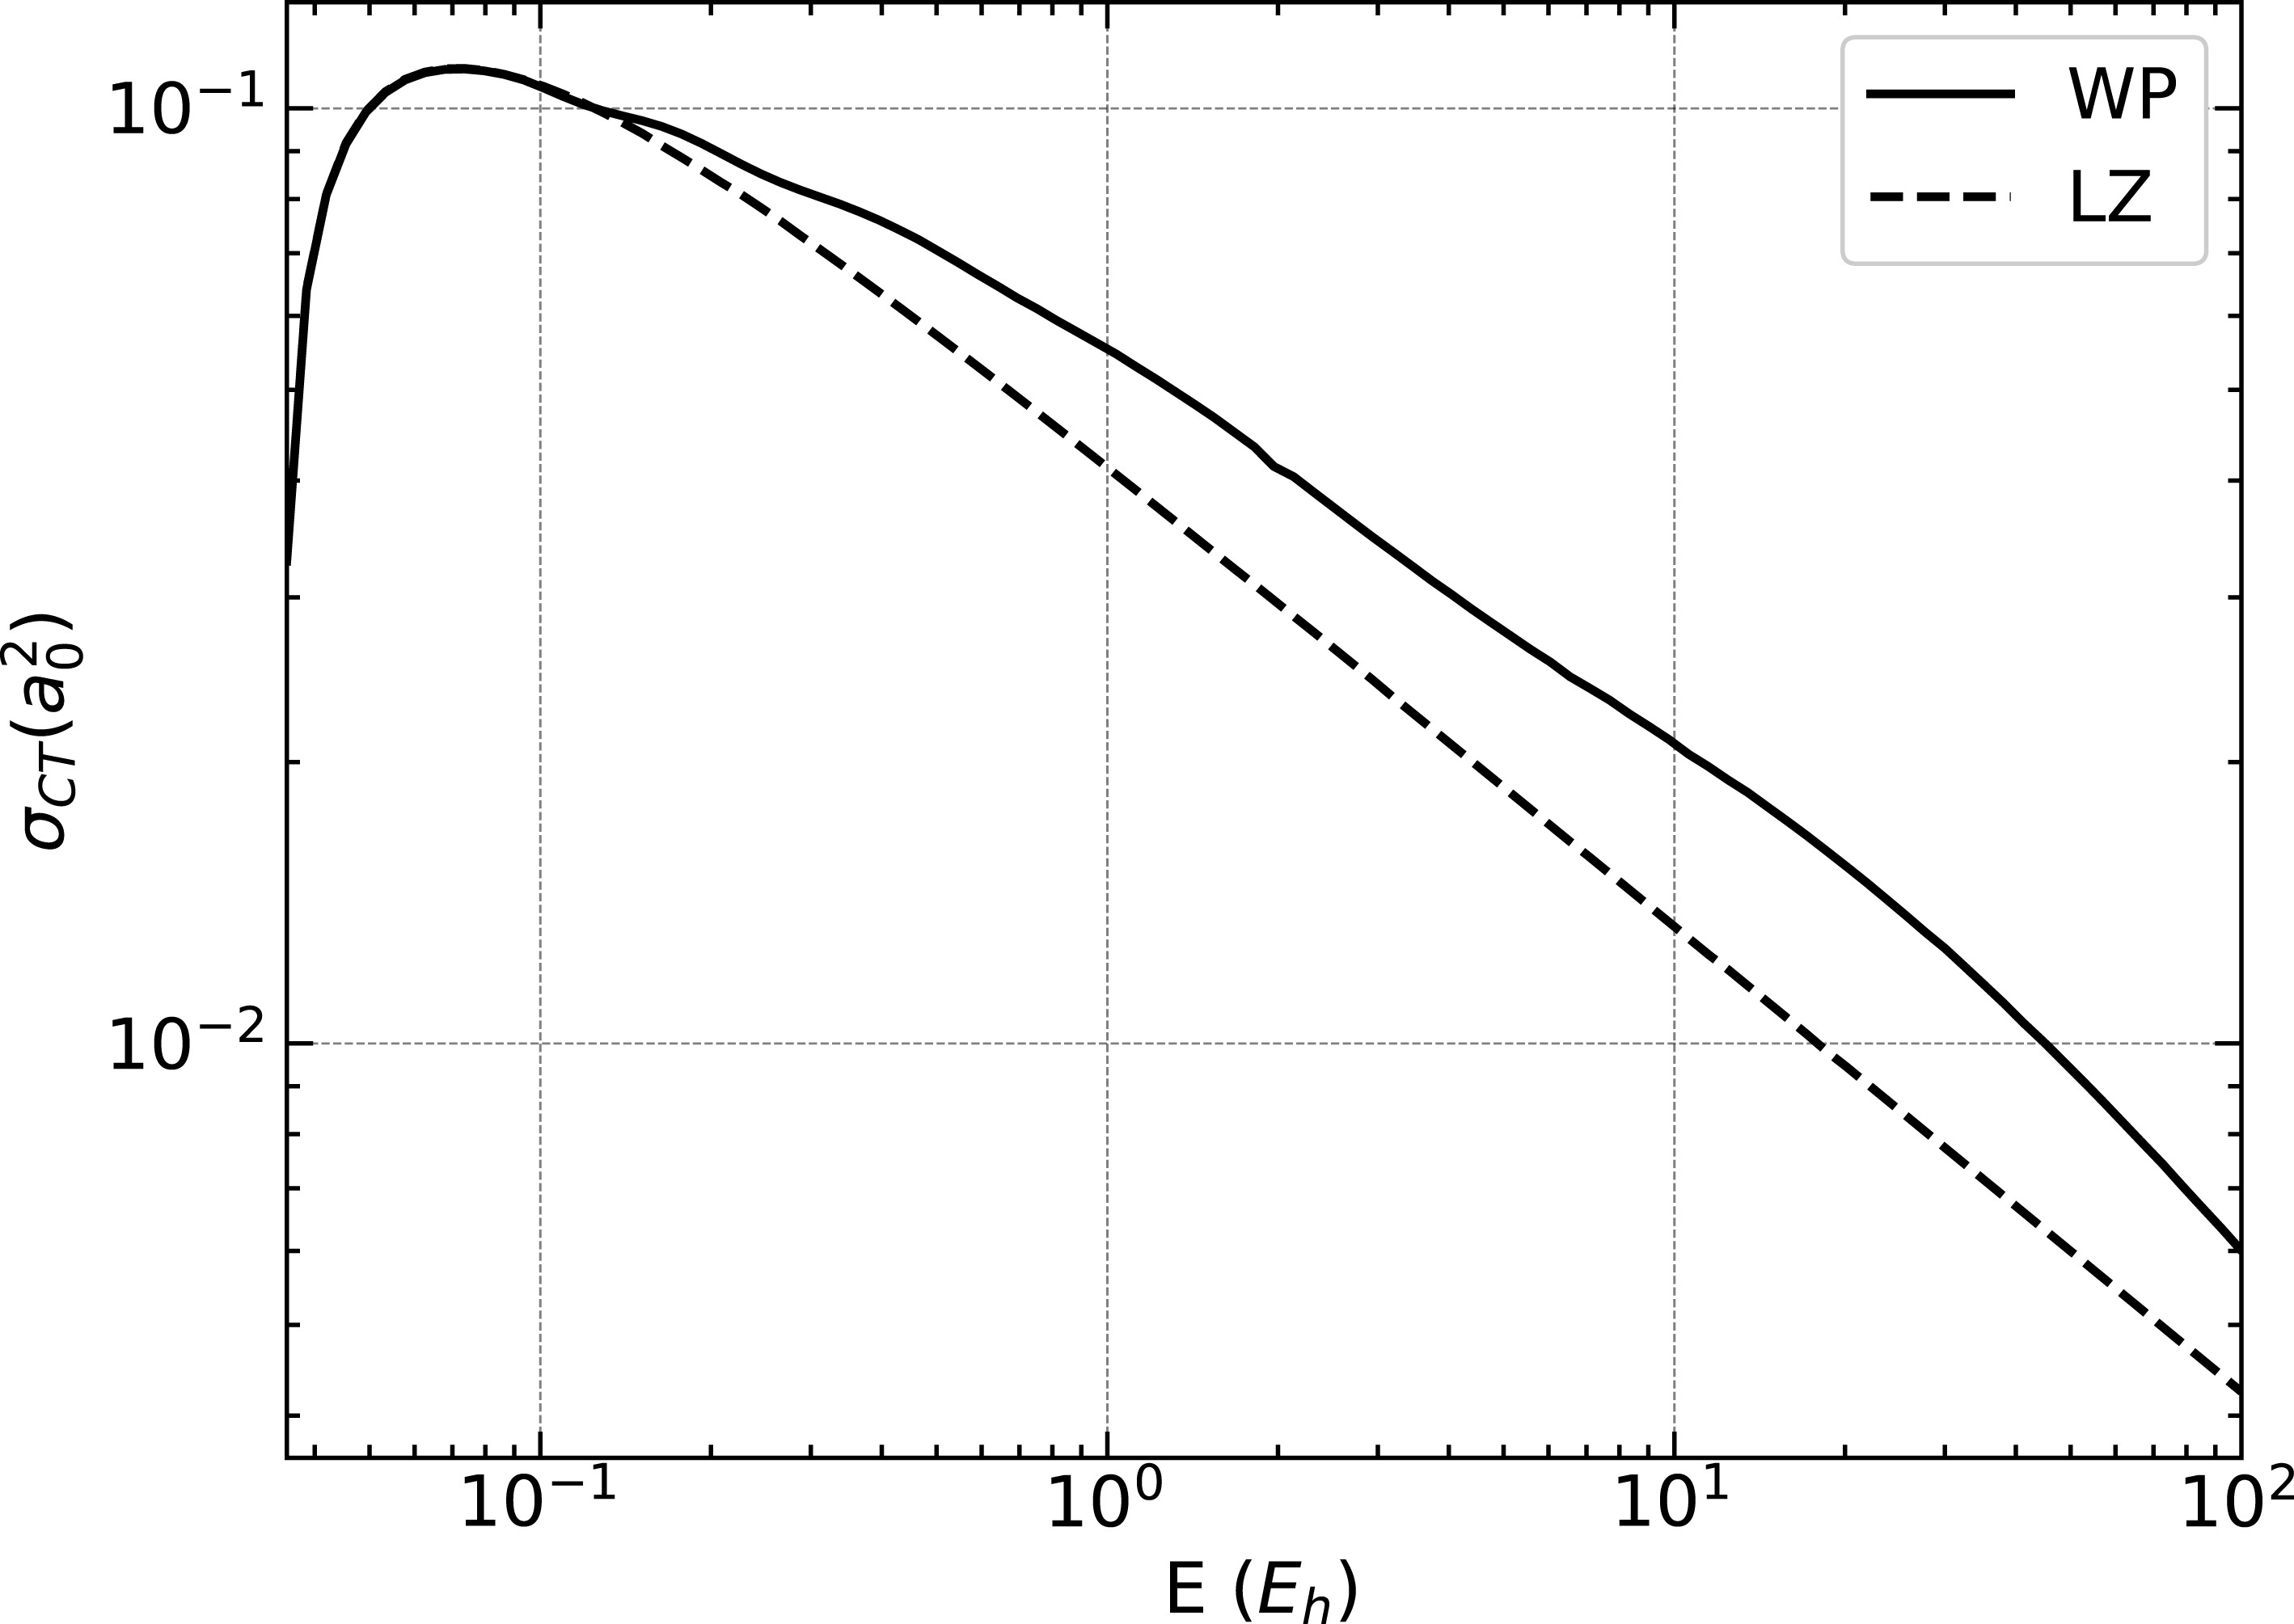
\includegraphics[width=\linewidth]{parts/02-Original_Research_and_Contributions/chapters/02-Primary_Scientific_Contributions/sections/images/1-s2.0-S0022407325003590-gr6_lrg}
\end{subfigure}\begin{subfigure}{.5\textwidth}
\centering
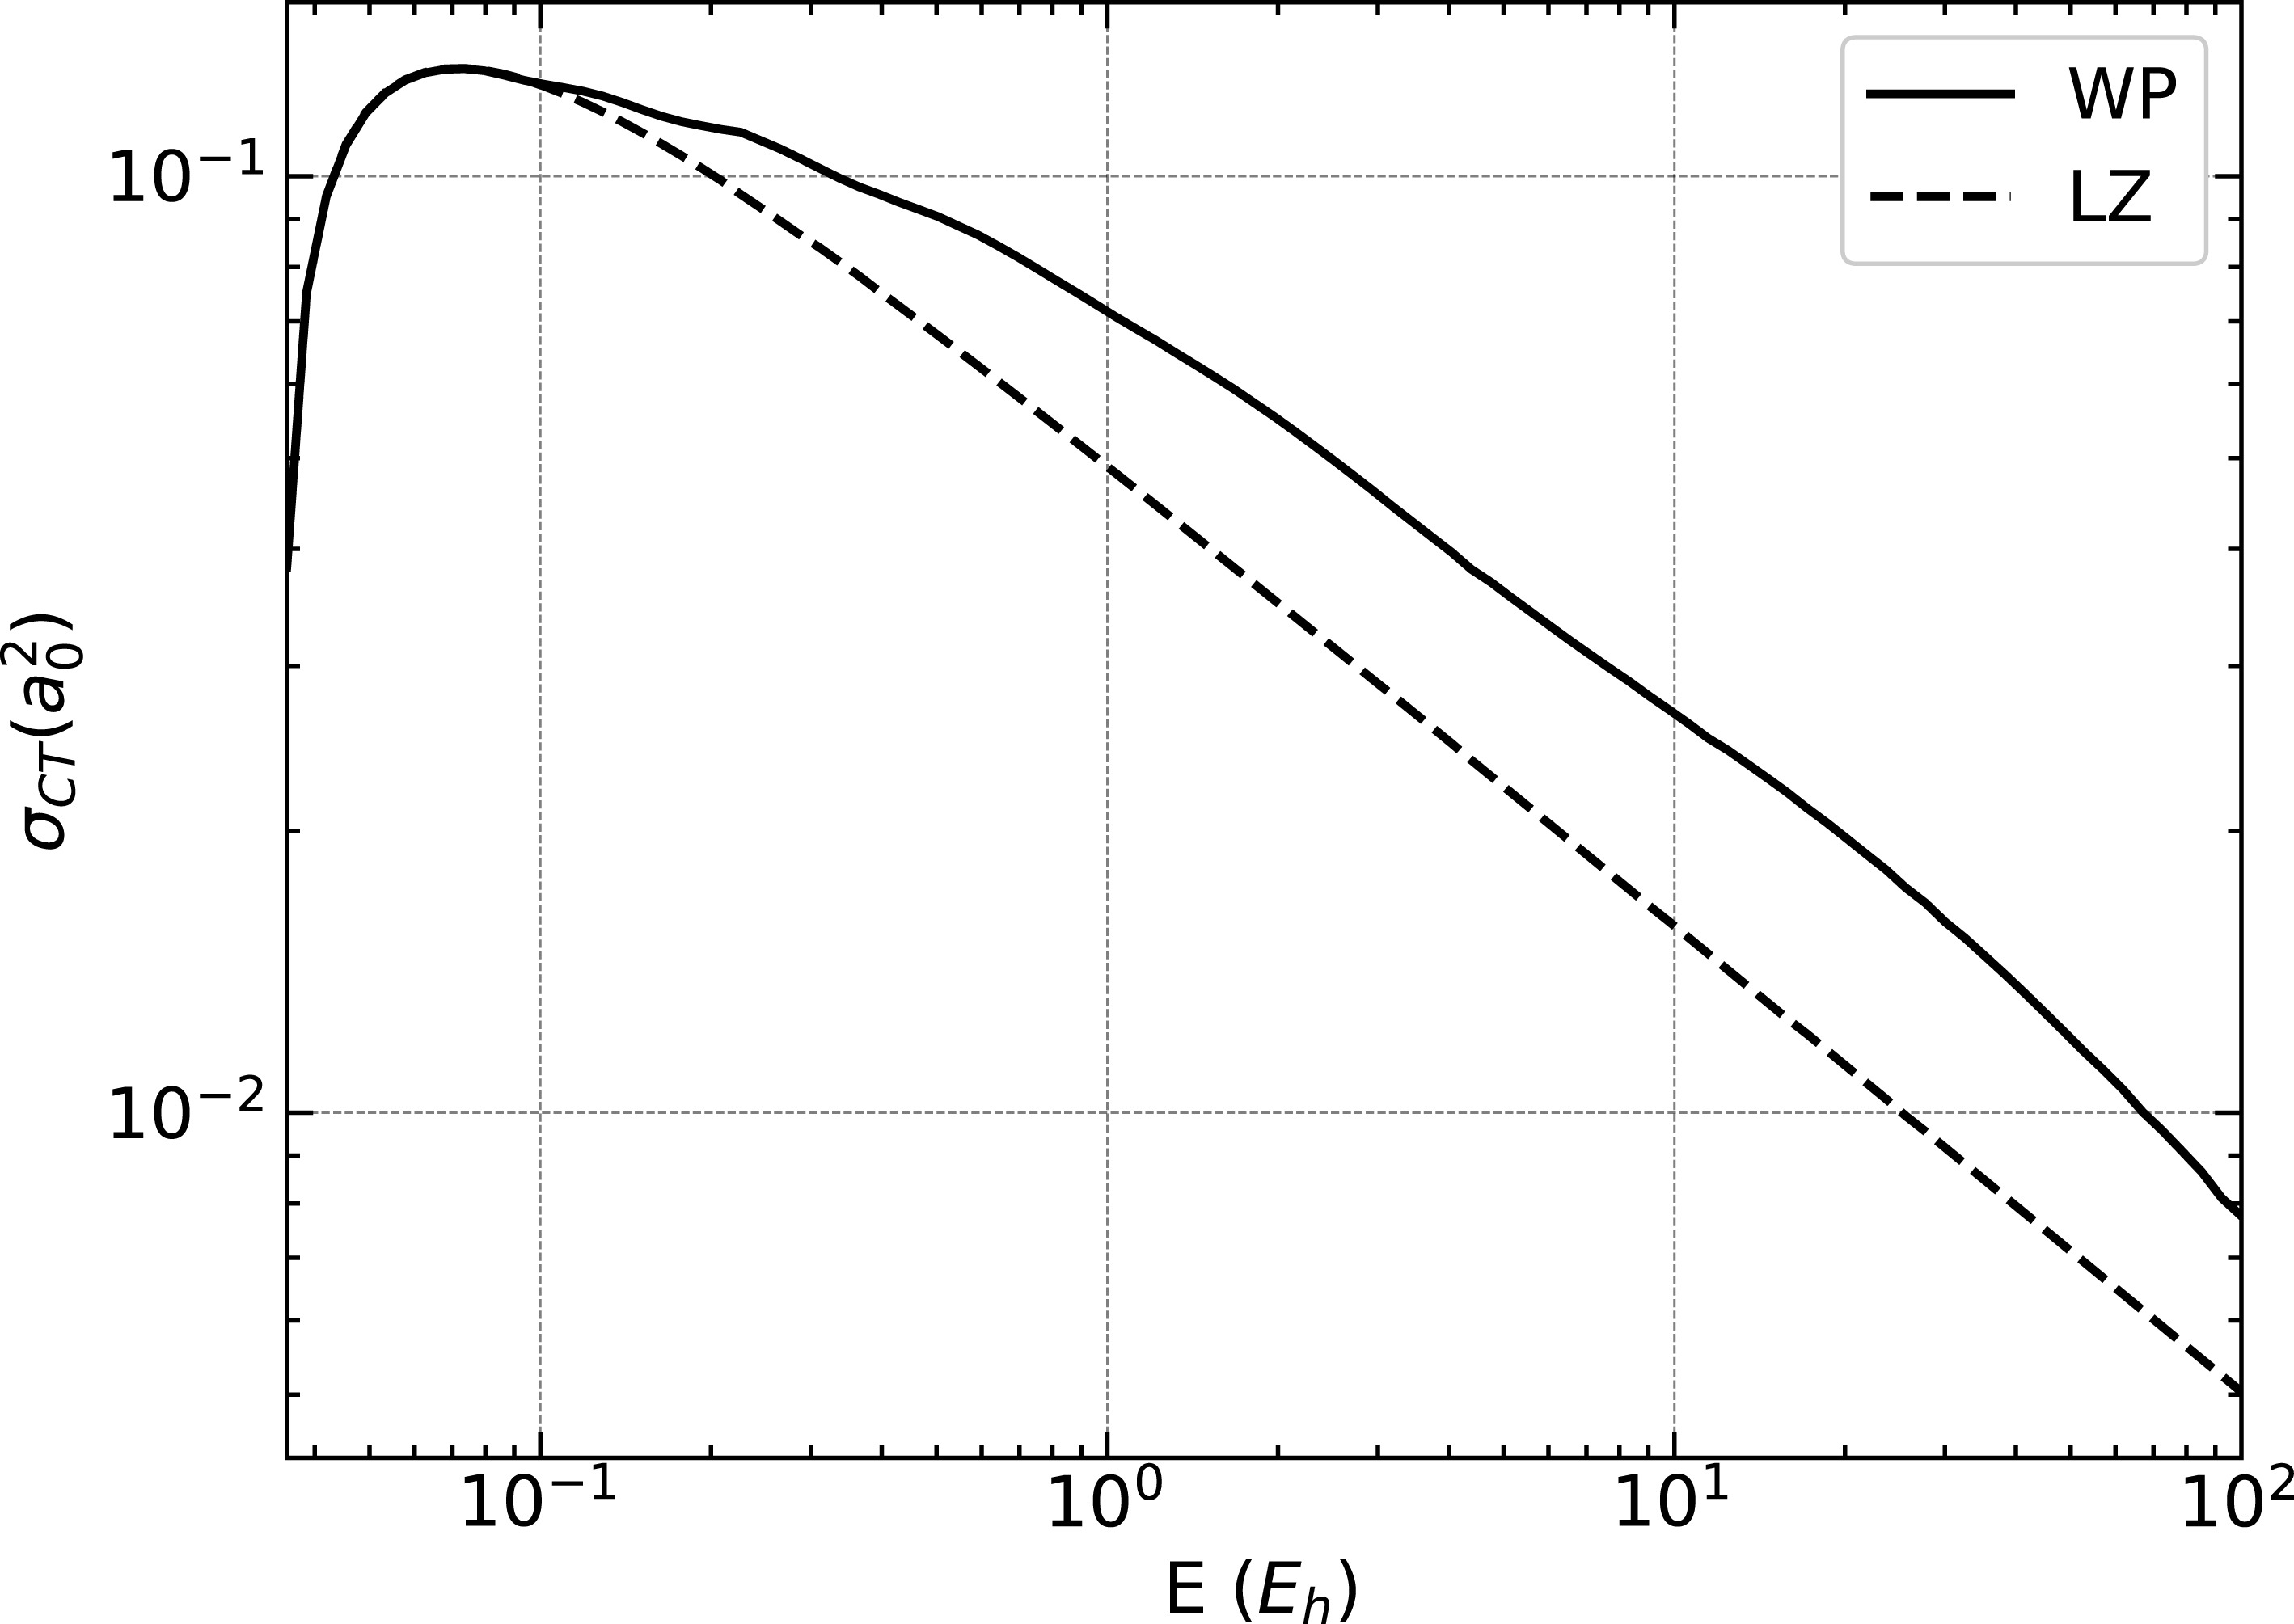
\includegraphics[width=\linewidth]{parts/02-Original_Research_and_Contributions/chapters/02-Primary_Scientific_Contributions/sections/images/1-s2.0-S0022407325003590-gr7_lrg}
\end{subfigure}
\caption{The charge transfer cross sections for the \ce{N-D^+} (left) and \ce{N-T^+} (right) systems as a function of collision energy. The WP label represents line obtained from the 1D quantum dynamics.}
\label{fig:soc_charge_transfer_cross_sections}
\end{figure}
Additionally, rate constants for the charge transfer process are calculated by integrating the cross sections over a Maxwell--Boltzmann distribution of collision energies as
\begin{equation}
k(T)=\sqrt{\frac{8}{\pi\mu(k_BT)^3}}\int_0^\infty E\sigma(E)\e^{-\frac{E}{k_BT}}\symrm{d}E,
\end{equation}
where $k_B$ is the Boltzmann constant, $T$ is the temperature and $\mu$ is the reduced mass of the system. The calculated rate constants are presented in Fig.~\ref{fig:soc_rate_constants} as a function of temperature.
\begin{figure}[!ht]
\centering
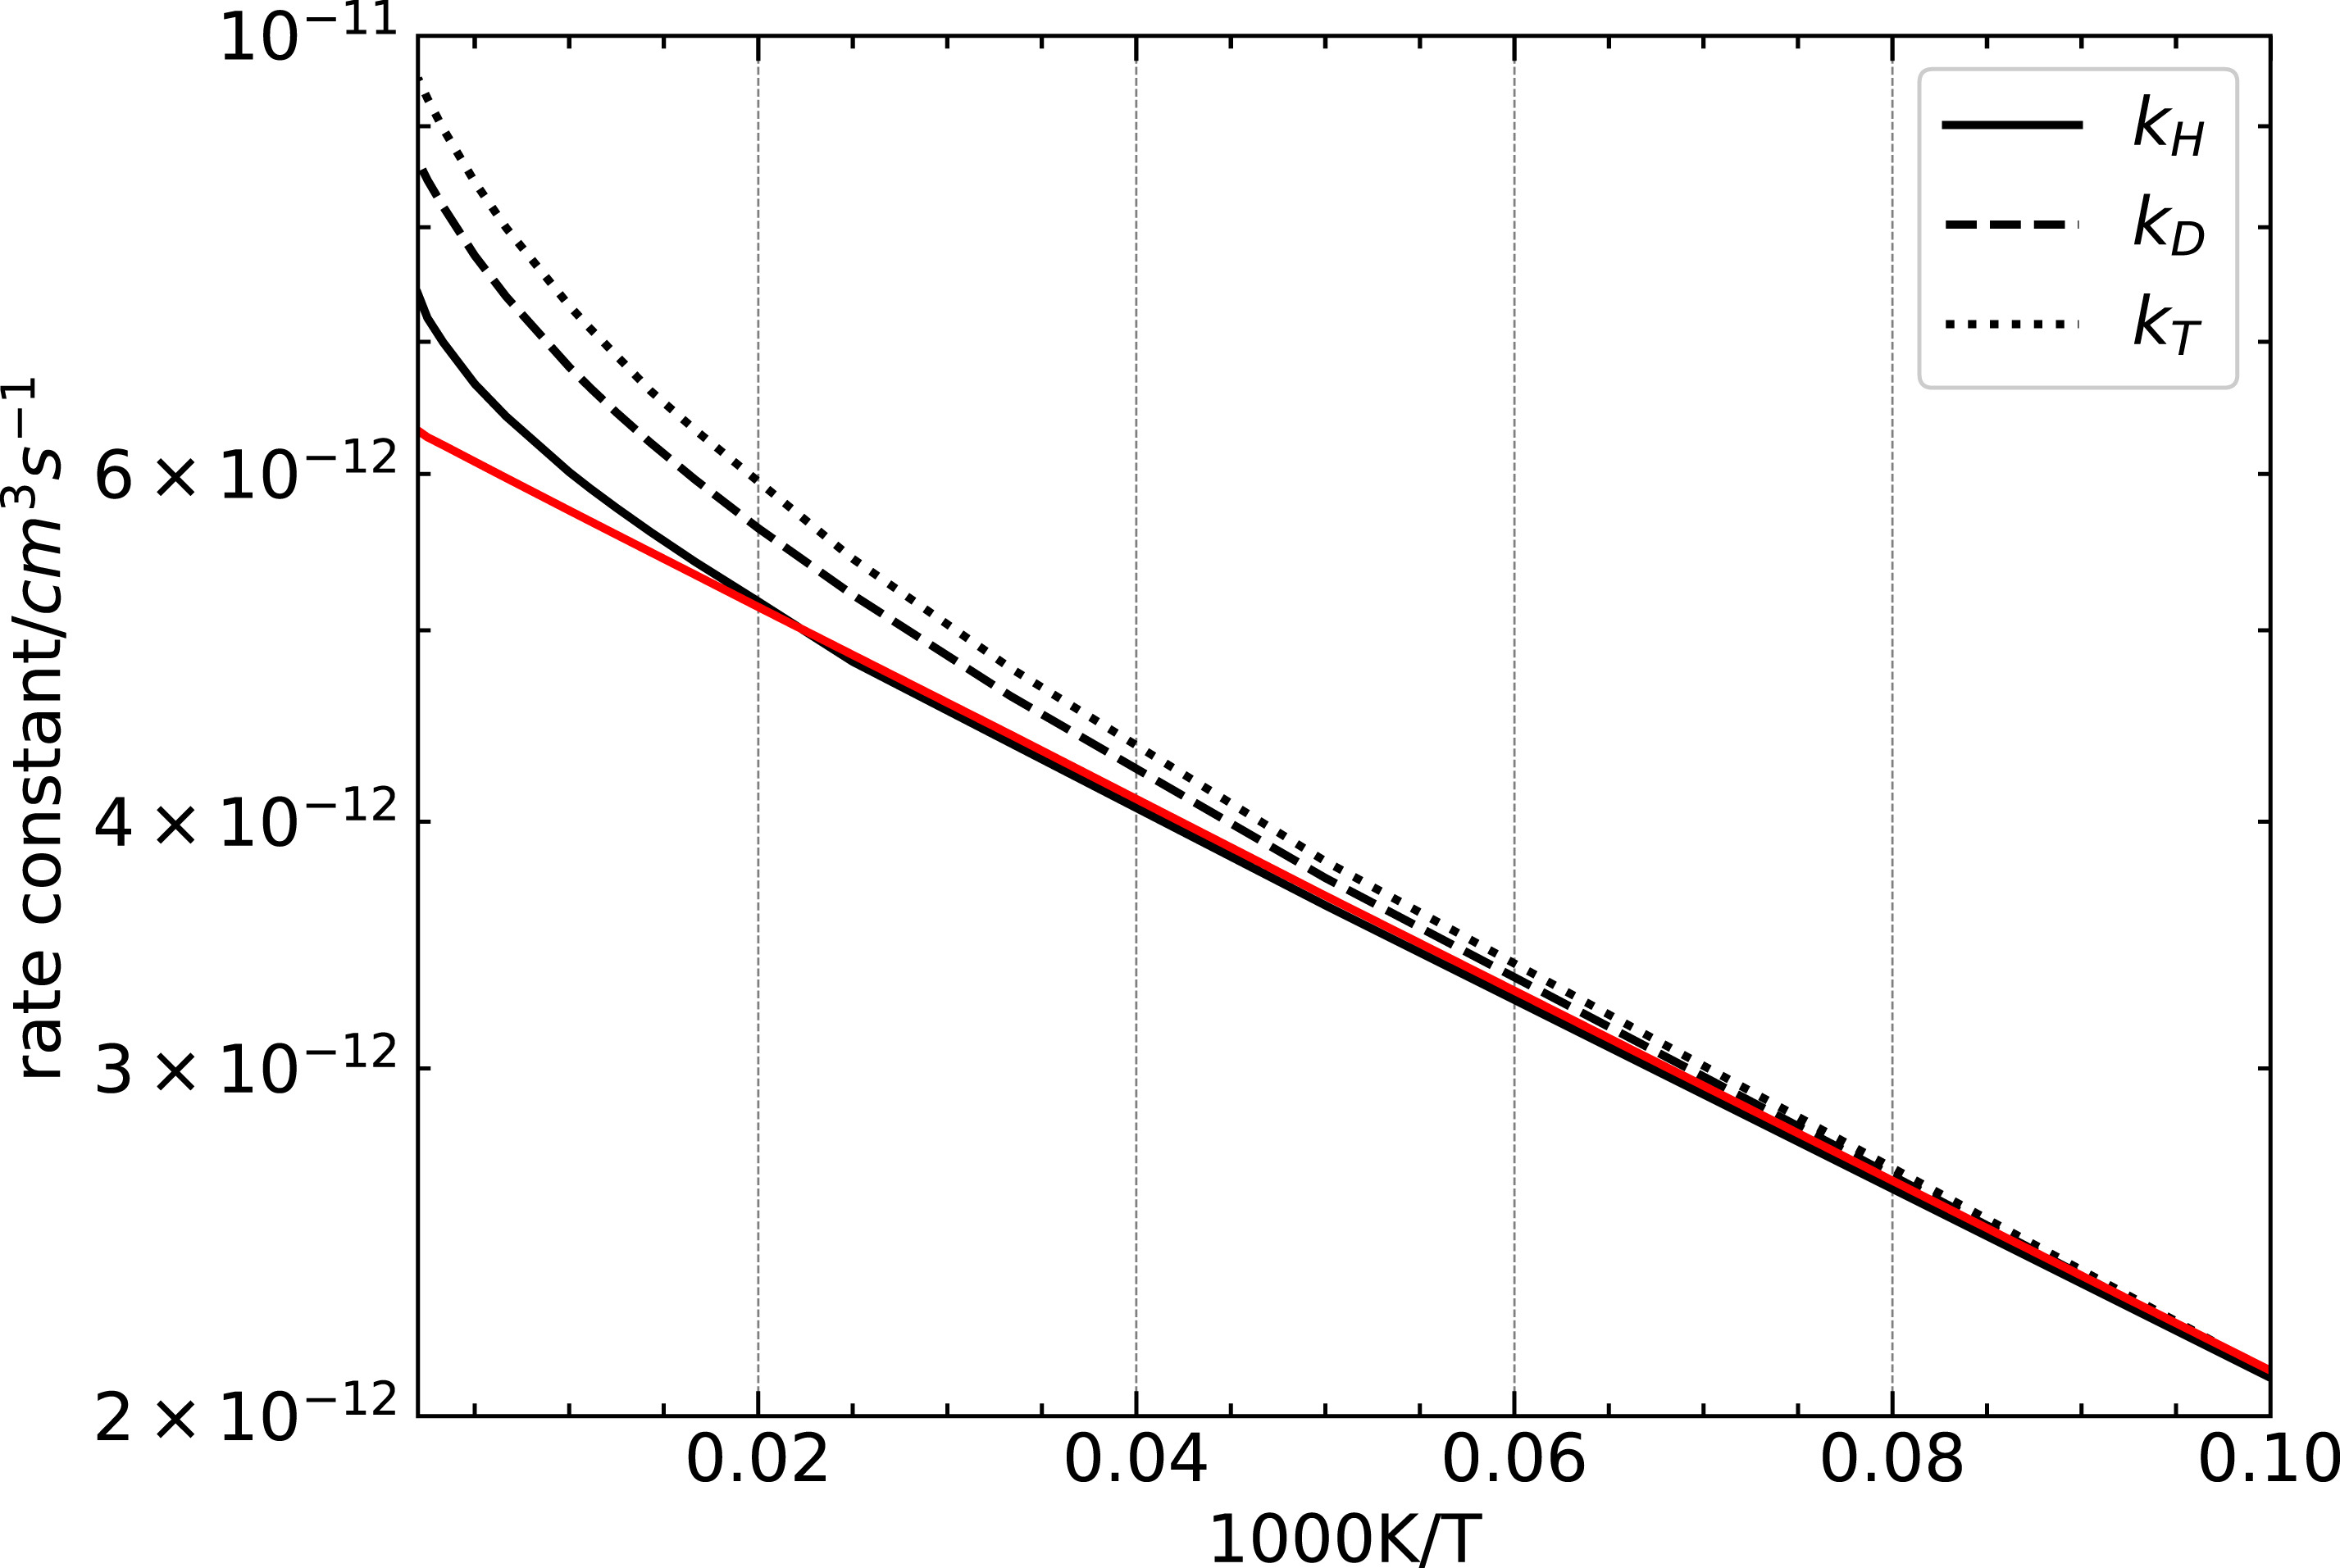
\includegraphics[width=0.7\linewidth]{parts/02-Original_Research_and_Contributions/chapters/02-Primary_Scientific_Contributions/sections/images/1-s2.0-S0022407325003590-gr10_lrg}
\caption{The rate constants for the collision reactions involving hydrogen ($k_H$), deuterium ($k_D$) and tritium ($k_T$) as a function of temperature. The straight red line represents the results from \acrshort{lz} theory for the hydrogen case.}
\label{fig:soc_rate_constants}
\end{figure}
Interestingly, when evaluating the thermal rate constants (Fig.~\ref{fig:soc_rate_constants}), the pronounced isotope effect observed in the cross sections almost entirely vanishes. This occurs because the increased cross section for heavier isotopes is perfectly compensated by the increased reduced mass ($\mu$) in the denominator of the rate constant equation. The rate constants exhibit strict Arrhenius behavior at lower temperatures, but the wavepacket data demonstrates a noticeable upward deviation at extremely high temperatures due to the short-range coupling effects accessed at high collision energies. Finally, this rigorous treatment definitively corrects the historical rate constants calculated, which were previously overestimated due to being erroneously derived from the barrierless reverse reaction. 
\subsection{Conclusion}
This study delivers a comprehensive, modernized investigation of spin-orbit induced charge transfer processes in \ce{H^+/D^+/T^+}-\ce{N(^4S)} collisions, effectively replacing the approximate, three-decade-old data with rigorous quantum dynamical results. Specifically, we learned that at high collision energies, the wavepacket penetrates the short-range region where the \acrshort{soc} is still significant, leading to a substantial increase in the charge transfer cross sections compared to the \acrshort{lz} theory. Furthermore, while the cross sections exhibit an isotope effect, the rate constants do not, due to the compensating effect of the reduced mass.

Within the broader context of this thesis, this work serves as the ultimate validation of the exact quantum dynamics algorithms developed and implemented in the custom \textsc{Zinq} package (detailed in Chapter~\ref{chp:supporting_numerical_studies}). The ability to perform rigorous quantum dynamics simulations for a complex, real-world system with strong \acrshort{soc} and to extract physically meaningful insights from these simulations demonstrates the reliability and robustness of the methods developed in this thesis.

Methodologically, this work demonstrates an unusual approach that combines computational chemistry methods with collision physics, elegantly combining high-level \textit{ab initio} electronic structure calculations with multidimensional quantum dynamics simulations. Practically, the resulting accurate cross sections and thermal rate constants for deuterium and tritium are important for astrophysical modeling and magnetic confinement fusion plasmas. By correcting obsolete approximations, this cross-disciplinary framework ensures that macroscopic transport codes, such as SOLPS-ITER, are now grounded in exact and rigorous quantum dynamics data.\supercite{10.1088/1741-4326/adcad0}

